\documentclass[10pt]{article}
\usepackage[english]{babel}
\usepackage{amsmath}
\usepackage{amssymb}
\usepackage{amsthm}
\usepackage{float}
\usepackage{tikz, tikzscale}
\usepackage{subcaption}
\usepackage[normalem]{ulem}
\usetikzlibrary{decorations.pathmorphing}
\usetikzlibrary{positioning}
\usetikzlibrary{calc}
\usepackage[colorlinks=true, allcolors=blue]{hyperref}
\usepackage{adjustbox}

\newtheorem{theorem}{Theorem}
\newtheorem{lemma}{Lemma}
\newtheorem{proposition}{Proposition}
\newtheorem{conjecture}{Conjecture}
\newtheorem{corollary}{Corollary}[theorem]

\theoremstyle{definition}
\newtheorem{definition}{Definition}
\newtheorem{remark}{Remark}
\newtheorem{example}{Example}

\DeclareMathOperator{\Ima}{Im}
\newcommand{\littletaller}{\mathchoice{\vphantom{\big|}}{}{}{}} % for the \restr command
\newcommand\restr[2]{{% we make the whole thing an ordinary symbol
    \left.\kern-\nulldelimiterspace % automatically resize the bar with \right
    #1 % the function
    \littletaller % pretend it's a little taller at normal size
    \right|_{#2} % this is the delimiter
}}

% Keywords command
\providecommand{\keywords}[1]
{
  \small
  \textbf{\textit{Keywords:}} #1
}

\title{$\alpha$-labeling of banana tree graphs}
\author{Borna Gojšić, Anamari Nakić}

\begin{document}

\maketitle

\begin{abstract}
  A banana tree graph, denoted by $B(n, k)$, is a tree constructed by connecting $n$ star graphs $S_k$ to a root vertex. This article builds upon previous research on graceful labelings of banana trees and explores their $\alpha$-labelability. We classify $\alpha$-labelings for $B(n, 1)$ and $B(1, k)$ trees. We present $\alpha$-labelings of the $B(n,k)$ tree, for $k \geq \frac{n}{2} + 1$ and $n \in \mathbb{N}$. Finally, we prove that the $B(n, k)$ tree is not $\alpha$-labelable for $1 < k \leq \frac{n}{2}$ and any $n \ge 3$.
\end{abstract}
\keywords{graph labeling; graceful labeling; $\alpha$-labeling; banana tree graph}

\section{Introduction}
An interesting problem of graceful labeling or $\beta$-labeling of a graph was first introduced by Rosa in \cite{R67}. A \textit{tree} is a graph in which any two vertices are connected by exactly one path. The question of whether a given tree allows a graceful labeling turned out to be a hard problem. A great open problem in graph theory is the Ringel-Kotzig conjecture that all trees are graceful. This topic has been a focus of many papers, an overview of many results can be found in famous dynamic survey by Gallian \cite{G97}.

In the same paper \cite{R67}, an $\alpha$-labeling (or a $\alpha$-valuation) was also defined as a graceful labeling with an additional property. Trees with $\alpha$-labelings have proven to be useful in the development of the theory of graph decompositions. Known results on this topic can also be found in \cite{G97} where open questions are also stated.

Banana tree $B(n, k)$, is a hierarchical tree constructed by connecting $n$ star graphs $S_k$ to a central vertex of the tree. They were introduced in \cite{CHY97}. It has been shown that banana trees and extended banana trees admit graceful labeling \cite{SJ09, SJ09b}.

\sout{Summary of Graceful Results G bananas [2566], [2565]

  Chen, Lu, and Yeh [639] define a firecracker as a graph obtained from the concatenation
  of stars by linking one leaf from each. They also define a banana tree as a graph obtained
  by connecting a vertex v to one leaf of each of any number of stars (v is not in any of the
  stars). They proved that firecrackers are graceful and conjecture that banana trees are
  graceful. Before Sethuraman and Jesintha [2566] and [2565] (see also [1242]) proved that
  all banana trees and extended banana trees (graphs obtained by joining a vertex to one
  leaf of each of any number of stars by a path of length of at least two) are graceful, various
  kinds of bananas trees had been shown to be graceful by Bhat-Nayak and Deshmukh [508],
by Murugan and Arumugam [2020], [2018] and by Vilfred [3093].}

However, the more restrictive nature of the $\alpha$-labelings of a tree motivates the question of whether all banana trees possess this property.
This paper investigates the $\alpha$-labelability of banana trees, presenting both theoretical and computational results. We provide explicit constructions for $\alpha$-labelings in certain cases, formulate conjectures regarding their existence for specific parameter ranges, and show non-existence results. With this paper we hope to contribute to the the study of graph labelings. Some of our generalization results were motivated by the work in \cite{MMK14}.

We will first show that all $B(n, 1)$ trees are $\alpha$-labelable for all $n \in \mathbb{N}$ as well as all $B(1, k)$ trees. We will then show that all $B(n, k)$ trees are $\alpha$-labelable for all $n \in \mathbb{N}$ and $k \geq \frac{n}{2} + 1$. Finally, we will show that all $B(n, k)$ trees are not $\alpha$-labelable for all $1 < k \le \frac{n}{2}$ and $n \geq 3$.

\section{Basic notions and results}

\begin{definition}
  A \textit{graph} $G = (V, E)$ is a pair of a nonempty finite set $V$  of vertices and a finite set $E$ of edges. An edge is an unordered pair of two vertices.
\end{definition}
An edge $e = \{v, w\}$ will be briefly denoted by $e = vw$ and we will say that the vertices $v$ and $w$ are \textit{adjacent} or \textit{neighboring}. Furthermore, we say that the edge $e$ is \textit{incident} to $v$ and $w$. We define the mapping $\deg_G: V(G) \rightarrow \mathbb{N}$ so that $\deg_G(v)$ is the number of adjacent vertices of $v$ in $G$, called the \textit{degree} of $v$. A \textit{leaf} is a vertex of degree 1.

A \textit{subgraph} $H$ of a graph $G$ is a graph such that $V(H) \subseteq V(G)$ and $E(H) \subseteq E(G)$. We say that $H$ is an \textit{induced subgraph} of $G$ if $E(H)$ consist of all of the edges from $E(G)$ that connect pairs of vertices in $V(H)$. A \textit{path} $P$ of a graph $G$ is an array of edges of the following form $v_1 v_2, v_2 v_3, \dots, v_{n-1} v_n$. The \textit{length of a path} $P$ is the number of edges. A path $P$ of length $n - 1$ in a graph $G$ can be viewed as a subgraph of $G$, and it is called \textit{a path graph} $P_n$. We say that a graph is \textit{connected} if there exists a path between any of its two vertices.

\begin{definition}
  A \textit{tree} is a graph in which any two vertices are connected by exactly one path. An equivalent definition is that a tree with $n$ vertices is a connected graph with $n - 1$ edges.
\end{definition}

Let us denote the set of integers from 1 to $n$ by $[n] := \{1,2,\dots,n\}$.
\begin{definition}
  Let $G = (V, E)$ be a graph with $n$ vertices and $m$ edges.
  A \textit{labeling} of $G$ is a mapping $f: V \rightarrow \mathbb{N}$. We say that a labeling is \textit{graceful} if $\Ima f \subseteq [m + 1]$, the induced edge labeling $f^*: E \rightarrow \mathbb{N}$ defined by
  $$
  f^*(vw) = |f(v) - f(w)|
  $$
  is injective and
  $$\Ima f^* = \{ f^*(vw) \, : \, vw \in E \} = [n-1].$$
  A labeling of $G$ is an \textit{$\alpha$-labeling} if it is graceful and if there exists a constant $\alpha \in \mathbb{N}$ such that
  $$ f(v) \leq \alpha < f(w) \mbox{ or }  f(w) \leq \alpha < f(v), \mbox{ for all } vw \in E.
  $$
  Other names for $\alpha$-labelings are \textit{balanced}, \textit{interlaced}, and \textit{strongly graceful}.
\end{definition}
A graph $G$ for which there exists an $\alpha$-labeling is said to be \textit{$\alpha$-labelable}. We say that two labelings $f$ and $g$ are \textit{isomorphic} if there exists an automorphism $\sigma: V \rightarrow V$ of $G$ such that $f = g \circ \sigma$. Two labelings are \textit{distinct} if and only if they are not isomorphic.

\begin{remark}  \cite{R77}
  \label{remark:alpha-labeling-properties}
  \begin{enumerate}
    \item If $f$ is an $\alpha$-labeling of $G$ and $f^*(vw) = 1$ for some $v, w \in V$, then $\alpha = \min\{f(v), f(w)\}$.
    \item If $f$ is an $\alpha$-labeling of a graph $G$ with $n$ vertices, then its complementary labeling $\overline{f}$ defined as $\overline{f}(v) = n + 1 - f(v)$ is also an $\alpha$-labeling of $G$ with $\overline{\alpha} = n - \alpha + 1$.
    \item If $f$ is an $\alpha$-labeling of $G$, its reverse (or inverse) labeling $f^r$ defined as
      $$
      f^r(v) =
      \begin{cases}
        \alpha + 1 - f(v), & f(v) \leq \alpha \\
        n + \alpha + 1 - f(v), & f(v) > \alpha
      \end{cases}
      $$
      is also an $\alpha$-labeling of $G$ with $\alpha^r = \alpha$.
  \end{enumerate}
\end{remark}

A star $S_k$ is the complete bipartite graph $K_{1,k}$, a tree with one internal node, \textit{the center} of the star, and $k$ leaves.

\begin{figure}[H]
  \centering
  \begin{subfigure}{0.24\textwidth}
    \centering
    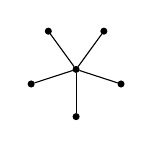
\begin{tikzpicture}[scale=0.3, every node/.style={circle, draw=black, fill=black, inner sep=0.75pt}]
      % Number of star graphs
      \def\nstars{1}
      % Leaves per star graph
      \def\leaves{5}
      % Radius for positioning leaves
      \def\radius{2}
      % Horizontal distance between star graphs
      \def\hstep{2.5}
      % Draw star graphs attached to the root node
      \foreach \i in {1,...,\nstars} {
        % Coordinates for the star's central node
        \node (c\i) at ({(\i-1)*\hstep - (\nstars-1)*\hstep/2}, 0) {};
        % Draw leaves around each star node
        \foreach \j in {1,...,\leaves} {
          \node (l\i\j) at ([shift={(270 - 360/\leaves + \j*360/\leaves: \radius)}] c\i) {};
          \draw (c\i) -- (l\i\j);
        }
      }
    \end{tikzpicture}
    \caption*{$S_6$}
  \end{subfigure}
  \begin{subfigure}{0.24\textwidth}
    \centering
    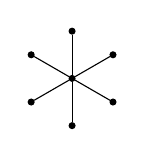
\begin{tikzpicture}[scale=0.3, every node/.style={circle, draw=black, fill=black, inner sep=0.75pt}]
      % Number of star graphs
      \def\nstars{1}
      % Leaves per star graph
      \def\leaves{6}
      % Radius for positioning leaves
      \def\radius{2}
      % Horizontal distance between star graphs
      \def\hstep{2.5}
      % Draw star graphs attached to the root node
      \foreach \i in {1,...,\nstars} {
        % Coordinates for the star's central node
        \node (c\i) at ({(\i-1)*\hstep - (\nstars-1)*\hstep/2}, 0) {};
        % Draw leaves around each star node
        \foreach \j in {1,...,\leaves} {
          \node (l\i\j) at ([shift={(270 - 360/\leaves + \j*360/\leaves: \radius)}] c\i) {};
          \draw (c\i) -- (l\i\j);
        }
      }
    \end{tikzpicture}
    \caption*{$S_7$}
  \end{subfigure}

  \caption{Examples of star trees}
  \label{fig:stars}
\end{figure}

\begin{definition}
  A \textit{banana tree} $B(n, k)$ is a tree obtained by joining a central vertex of the tree, \textit{the root}, with one leaf of each of the $n$ copies of a star graph $S_k$.
\end{definition}
From the definition for $k = 1$, we can see that $B(n,1) \cong K_{1, n} \cong S_n$. Examples of $B(n, k)$ for $k > 2 $ trees are shown in Figure \ref{fig:banana-trees}.
\begin{figure}[H]
  \centering
  \begin{subfigure}{0.125\textwidth}
    \centering
    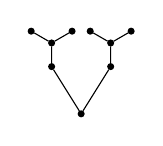
\begin{tikzpicture}[scale=0.3, every node/.style={circle, draw=black, fill=black, inner sep=0.75pt}]

      % Root node
      \node (root) at (0, -3) {};

      % Number of star graphs
      \def\nstars{2}

      % Leaves per star graph
      \def\leaves{3}

      % Radius for positioning leaves
      \def\radius{1}

      % Horizontal distance between star graphs
      \def\hstep{2.5}

      % Draw star graphs attached to the root node
      \foreach \i in {1,...,\nstars} {
        % Coordinates for the star's central node
        \node (c\i) at ({(\i-1)*\hstep - (\nstars-1)*\hstep/2}, 0) {};

        % Draw leaves around each star node
        \foreach \j in {1,...,\leaves} {
          \node (l\i\j) at ([shift={(270 - 360/\leaves + \j*360/\leaves: \radius)}] c\i) {};
          \draw (c\i) -- (l\i\j);
        }

        % Find the lowest leaf (typically the one at 270 degrees)
        \draw (root) -- (l\i1);
      }

    \end{tikzpicture}
    \caption*{$B(2, 4)$}
  \end{subfigure}
  \hspace*{1cm}
  \begin{subfigure}{0.15\textwidth}
    \centering
    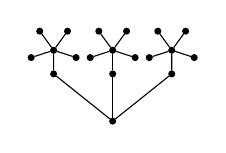
\begin{tikzpicture}[scale=0.3, every node/.style={circle, draw=black, fill=black, inner sep=0.75pt}]

      % Root node
      \node (root) at (0, -3) {};

      % Number of star graphs
      \def\nstars{3}

      % Leaves per star graph
      \def\leaves{5}

      % Radius for positioning leaves
      \def\radius{1}

      % Horizontal distance between star graphs
      \def\hstep{2.5}

      % Draw star graphs attached to the root node
      \foreach \i in {1,...,\nstars} {
        % Coordinates for the star's central node
        \node (c\i) at ({(\i-1)*\hstep - (\nstars-1)*\hstep/2}, 0) {};

        % Draw leaves around each star node
        \foreach \j in {1,...,\leaves} {
          \node (l\i\j) at ([shift={(270 - 360/\leaves + \j*360/\leaves: \radius)}] c\i) {};
          \draw (c\i) -- (l\i\j);
        }

        % Find the lowest leaf (typically the one at 270 degrees)
        \draw (root) -- (l\i1);
      }

    \end{tikzpicture}
    \caption*{$B(3, 6)$}
  \end{subfigure}
  \hspace*{1cm}
  \begin{subfigure}{0.2\textwidth}
    \centering
    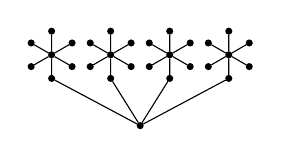
\begin{tikzpicture}[scale=0.3, every node/.style={circle, draw=black, fill=black, inner sep=0.75pt}]

      % Root node
      \node (root) at (0, -3) {};

      % Number of star graphs
      \def\nstars{4}

      % Leaves per star graph
      \def\leaves{6}

      % Radius for positioning leaves
      \def\radius{1}

      % Horizontal distance between star graphs
      \def\hstep{2.5}

      % Draw star graphs attached to the root node
      \foreach \i in {1,...,\nstars} {
        % Coordinates for the star's central node
        \node (c\i) at ({(\i-1)*\hstep - (\nstars-1)*\hstep/2}, 0) {};

        % Draw leaves around each star node
        \foreach \j in {1,...,\leaves} {
          \node (l\i\j) at ([shift={(270 - 360/\leaves + \j*360/\leaves: \radius)}] c\i) {};
          \draw (c\i) -- (l\i\j);
        }

        % Find the lowest leaf (typically the one at 270 degrees)
        \draw (root) -- (l\i1);
      }
    \end{tikzpicture}
    \caption*{$B(4, 7)$}
  \end{subfigure}
  \caption{Examples of $B(n,k)$ trees}
  \label{fig:banana-trees}
\end{figure}

\subsection{Rooted Standard Form of a Banana Tree}

A \textit{rooted standard form} of a $B(n, k)$ tree is a way of representing the tree by specifically naming the vertices. This form of representing the $B(n,k)$ tree is motivated by its symmetries and the results on $\alpha$-labelings we obtained. A general $B(n, k)$ tree in this form is shown in Figure \ref{fig:rsf-banana-tree}.

\begin{figure}[H]
  \centering
  \begin{adjustbox}{center}
    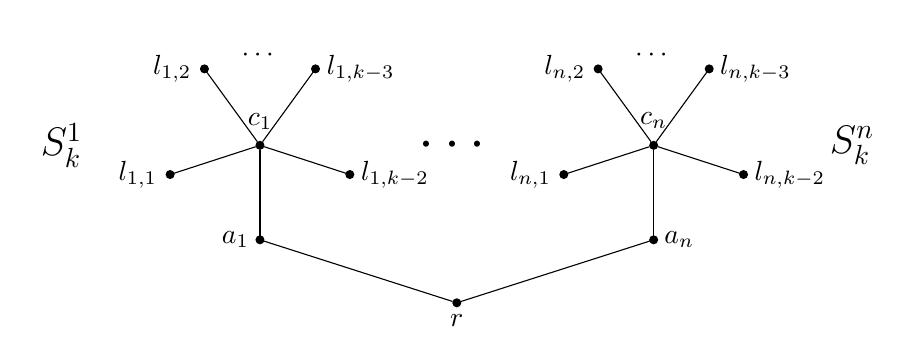
\begin{tikzpicture}[scale=1, every node/.style={circle, draw, fill=black, inner sep=1pt}]

      \node[label=below:{$r$}] (central) at (0, -2) {};

      \def\k{5} % Number of leaves in each star graph
      \def\leafradius{1.2} % Radius of the circular arrangement of leaves

      \node[label=above:{$c_1$}] (b1) at (-2.5, 0) {};
      \node[label=above:{$c_n$}] (b2) at (2.5, 0) {};

      \foreach \j in {1,...,\k} {
        \pgfmathsetmacro\leafangle{-90 - 360/\k * (\j-1)}

        \coordinate (l1\j) at ($(b1) + (\leafangle:\leafradius)$);
        \coordinate (l2\j) at ($(b2) + (\leafangle:\leafradius)$);
      }

      \node[label=left:{$a_1$}] at (l11) {};
      \node[label=left:{$l_{1,1}$}] at (l12) {};
      \node[label=left:{$l_{1,2}$}] at (l13) {};
      \node[label=right:{$l_{1,k-3}$}] at (l14) {};
      \node[label=right:{$l_{1,k-2}$}] at (l15) {};

      \draw (b1) -- (l11);
      \draw (b1) -- (l12);
      \draw (b1) -- (l13);
      \draw (b1) -- (l14);
      \draw (b1) -- (l15);

      \node[label=right:{$a_n$}] at (l21) {};
      \node[label=left:{$l_{n,1}$}] at (l22) {};
      \node[label=left:{$l_{n,2}$}] at (l23) {};
      \node[label=right:{$l_{n,k-3}$}] at (l24) {};
      \node[label=right:{$l_{n,k-2}$}] at (l25) {};

      \draw (b2) -- (l21);
      \draw (b2) -- (l22);
      \draw (b2) -- (l23);
      \draw (b2) -- (l24);
      \draw (b2) -- (l25);

      \foreach \j in {1,...,2} {
        \pgfmathsetmacro\dotangle{90}
        \node[draw=none, fill=none] at ($(b\j) + (\dotangle:0.95*\leafradius)$) {\textbf{$\cdots$}};
      }

      \node[draw=none, fill=none] at ($(b1) + (180:2.1*\leafradius)$) {\Large \textbf{$S^1_k$}};
      \node[draw=none, fill=none] at ($(b2) + (0:2.1*\leafradius)$) {\Large \textbf{$S^n_k$}};

      \draw (central) -- (l11);
      \draw (central) -- (l21);

      % Optional: add dots to indicate missing parts in the middle
      \node[draw=none,fill=none] at (0,0) {\huge \textbf{$\cdots$}};

    \end{tikzpicture}
  \end{adjustbox}

  \caption{Rooted standard form of a $B(n, k)$ tree}
  \label{fig:rsf-banana-tree}
\end{figure}
In this representation the vertex set of a $B(n, k )$ tree for $k > 1$ is
$$
V(B(n,k)) = \{r\} \cup \{ a_i \mid i \in [n]\} \cup \{c_i \mid i \in [n] \} \cup \{l_{i,j} \mid i \in [n], j \in [k-2] \}.
$$
The vertex we named $r$ is the root of $B(n,k)$, the vertices $a_i$ are adjacent to the root and $c_i$ are the centers of the stars $S^i_k$, the induced $i$-th star subgraph of $B(n, k)$. To improve the readability of the paper later on, we introduce the following notation for two subsets of vertices of $S^i_k$ : $\mathcal{L}_i = \{l_{i,j} \mid j \in [k-2] \}$ and $\mathcal{B}_i$ = $\{a_i\} \cup \mathcal{L}_i$. We remark that swapping the labelings of two stars $S^i_k$ and $S^{i'}_k$ does not change the labeling of $B(n,k)$. Also, swapping the labels of any two leaves $l_{i, j}$ and $l_{i, j'}$ of $S^i_k$ does not change the labeling of $B(n,k)$. The edge set is
$$
E(B(n,k)) = \{r a_i \mid i \in [n]\} \cup \{a_i c_i \mid i \in [n]\} \cup \{c_i l_{i,j} \mid i \in [n], j \in [k-2]\}.
$$
When $k = 1$, the vertex set is
$$
V(B(n,1)) = \{r\} \cup \{ a_i \mid i \in [n]\}
$$
and the edge set is
$$
E(B(n,1)) = \{r a_i \mid i \in [n]\}.
$$
The $B(n, k)$ tree has $n k + 1$ vertices and $n k$ edges.

\section{\texorpdfstring{$\alpha$}{Alpha}-labelings of a \texorpdfstring{$B(n,k)$}{B(n,k)} tree}
Let $f : V \rightarrow \mathbb{N}$ be a labeling of a $B(n, k)$ tree. For an arbitrary set of vertices $S$ of $B(n, k)$ tree we will write
$$
\mathcal{F}(S) = \Ima \restr{f}{S} = \{f(x) \mid x \in S\}.
$$
Also, we will write just $\mathcal{F}$ when we are looking at values of $f$ across the whole domain, i.e. $\mathcal{F} = \Ima f$.

\begin{definition}
  Let $\mathcal{A}(n,k)$ be the set of all $\alpha$-labelings of the $B(n,k)$ tree and $\mathcal{A}_x(n,k)$ be the set of all $\alpha$-labelings of the $B(n,k)$ tree where $f(r) = x$. Also, we will use the notation $A(n,k) = |\mathcal{A}(n,k)|$ and $A_x(n,k) = |\mathcal{A}_x(n,k)|$.
\end{definition}

\begin{proposition}
  \label{proposition:RC}
  Let $f$ be an $\alpha$-labeling of the $B(n,k)$ tree for any $n \in \mathbb{N}$ and $k \ge 2$. Then,
  $$
  f(r) \le \alpha \iff f(c_i) \le \alpha \quad \forall i \in [n]
  $$
\end{proposition}

\begin{proof}
  ($\Leftarrow$): Let $f(c_i) \le \alpha$ for all $i \in [n]$. Then, since $f$ is an $\alpha$-labeling and $c_i a_i$ is an edge of the $B(n,k)$ tree for all $i \in [n]$, we have $f(c_i) \le \alpha < f(a_i)$ for all $i \in [n]$. Furthermore, since $r a_i$ is an edge of the $B(n, k)$ tree for all $i \in [n]$, we must have $f(r) \le \alpha < f(a_i)$, and thus we have proven one direction of the equivalence.

  ($\Rightarrow$): Let $f(r) \le \alpha$. Then, we must have $f(r) \le \alpha < f(a_i)$ for all $i \in [n]$, since $f$ is an $\alpha$-labeling and $r a_i$ is an edge of the $B(n, k)$ tree for all $i \in [n]$. Furthermore, we must have $f(c_i) \le \alpha < f(a_i)$ for all $i \in [n]$, since $f$ is an $\alpha$-labeling and $c_i a_i$ is an edge of the $B(n,k)$ tree for all $i \in [n]$.
\end{proof}

\begin{theorem}
  \label{thm:partition}
  Let $f$ be an $\alpha$-labeling of the $B(n,k)$ tree for any $n \in \mathbb{N}$ and $k \ge 2$. Then, exactly one of the following holds:

  \begin{enumerate}
    \item $\mathcal{F}(RC) = [n + 1]$ and $\alpha = n + 1$, or
    \item $\mathcal{F}(RC) = \{nk + 1, nk, \dots, nk + 1 - n\}$ and $\alpha = nk - n$,
  \end{enumerate}

  where $RC = \{r\} \cup \{c_i \mid i \in [n]\}$.
\end{theorem}

\begin{proof}
  By Proposition \ref{proposition:RC} we have that
  $$
  f(r) \le \alpha \iff f(c_i) \le \alpha \quad \forall i \in [n]
  $$
  Therefore, we will look at the two cases: when $f(r) \le \alpha$ and when $f(r) > \alpha$.
  \begin{enumerate}
    \item Let $f(r) \le \alpha$. Then, we have $f(c_i) \le \alpha$ for all $i \in [n]$. We must have $f(v) > \alpha$ for all $v \in V \setminus RC$, since for every $v \in V \setminus RC$, $v c_i$ is an edge of $B(n, k)$ for some $i \in [n]$. Thus, we have exactly $|RC| = n + 1$ numbers that are $\le \alpha$. Therefore, we have $\alpha = n + 1$.

    \item Let $f(r) > \alpha$. Then, we have $f(c_i) > \alpha$ for all $i \in [n]$. We must have $f(v) \le \alpha$ for all $v \in V \setminus RC$, since for every $v \in V \setminus RC$, $v c_i$ is an edge of $B(n, k)$ for some $i \in [n]$. Thus, we have exactly $|V \setminus RC| = nk + 1 - n + 1 = nk - n$ numbers that are $\le \alpha$. Therefore, we have $\alpha = nk - n$.
  \end{enumerate}
\end{proof}

\begin{theorem}
  \label{thm:complementarity}
  For every $n, k \in \mathbb{N}$, we have
  $$
  \overline{\mathcal{A}_x}(n, k) = \mathcal{A}_{nk + 2 - x}(n, k),
  $$
  where $\overline{\mathcal{A}_x}(n, k) = \{\overline{f} : f \in \mathcal{A}_x(n, k)\}$
\end{theorem}

\begin{proof}
  Let $f \in \mathcal{A}_x(n, k)$ be an $\alpha$-labeling of the $B(n, k)$ tree with $f(r) = x$. Then, by Remark \ref{remark:alpha-labeling-properties}, we have that $\overline{f}(v) = n + 1 - f(v)$ for all $v \in V(B(n, k))$ and it is an $\alpha$-labeling. Thus, we have $\overline{f}(r) = nk + 2 - x$ and therefore,
  $$
  \overline{\mathcal{A}_x}(n, k) \subseteq \mathcal{A}_{nk + 2 - x}(n, k)
  $$
  Analogously, let $g \in \mathcal{A}_{nk + 2 - x}(n, k)$ be an $\alpha$-labeling of the $B(n, k)$ tree with $g(r) = nk + 2 - x$. Then, we have that $\overline{g}(v) = n + 1 - g(v)$ for all $v \in V(B(n, k))$. Thus, we have $\overline{g}(r) = x$ and therefore,
  $$
  \mathcal{A}_{nk + 2 - x}(n, k) \subseteq \overline{\mathcal{A}_x}(n, k)
  $$
  Finally, we have that $\overline{\mathcal{A}_x}(n, k) = \mathcal{A}_{nk + 2 - x}(n, k)$.
\end{proof}

\begin{corollary}
  For every $n, k \in \mathbb{N}$, we have
  $$
  \mathcal{A}(n, k) = \bigcup_{x = 1}^{n + 1} (\mathcal{A}_x(n, k) \cup \overline{\mathcal{A}_x}(n, k))
  $$
\end{corollary}

\begin{proof}
  Since we have that $\mathcal{F}(RC)$ is either $[n + 1]$ or $\{nk + 1, nk, \dots, nk + 1 - n\}$, we know that the following holds:
  $$
  \mathcal{A}(n, k) = \left(\bigcup_{x = 1}^{n + 1} \mathcal{A}_x(n, k)\right) \cup \left(\bigcup_{x = nk + 1 - n}^{nk + 1} \mathcal{A}_x(n, k)\right)
  $$
  Then, by Theorem \ref{thm:complementarity}, we have
  \begin{align*}
    \mathcal{A}(n, k) &= \left(\bigcup_{x = 1}^{n + 1} \mathcal{A}_x(n, k)\right) \cup \left(\bigcup_{x = 1}^{n + 1} \overline{\mathcal{A}_x}(n, k)\right)\\
    &= \bigcup_{x = 1}^{n + 1} (\mathcal{A}_x(n, k) \cup \overline{\mathcal{A}_x}(n, k)) \\
  \end{align*}
\end{proof}

\begin{corollary}
  For every $n \in \mathbb{N}$ and $k \ge 2$, we have
  $$
  A(n, k) = 2 \sum_{x = 1}^{n + 1} A_x(n, k)
  $$
\end{corollary}

\begin{proof}
  By the previous corollary, we have that
  \begin{align*}
    A(n, k) &= |\mathcal{A}(n, k)| = \left|\bigcup_{x = 1}^{n + 1} (\mathcal{A}_x(n, k) \cup \overline{\mathcal{A}_x}(n, k))\right|\\
    &= \sum_{x = 1}^{n + 1} |\mathcal{A}_x(n, k)| + |\overline{\mathcal{A}_x}(n, k)| = 2 \sum_{x = 1}^{n + 1} A_x(n, k)
  \end{align*}
\end{proof}

\begin{theorem}
  \label{thm:reversability}
  For every $n, k \in \mathbb{N}$ and $x \in [n + 1]$, we have
  $$
  \mathcal{A}^r_x(n, k) = \mathcal{A}_{n + 2 - x}(n, k),
  $$
  where $\mathcal{A}^r_x(n, k) = \{f^r : f \in \mathcal{A}_x(n, k)\}$.
\end{theorem}

\begin{proof}
  Let $f \in \mathcal{A}_x(n, k)$ be an $\alpha$-labeling of the $B(n, k)$ tree with $f(r) = x \in [n + 1]$. Then, by Remark \ref{remark:alpha-labeling-properties}, we have that $f^r(v) = n + 2 - f(v)$ for all $v \in RC$, since $\alpha = n + 1$. Thus, we have $f^r(r) = n + 2 - x$ and therefore,
  $$
  \mathcal{A}^r_x(n, k) \subseteq \mathcal{A}_{n + 2 - x}(n, k).
  $$
  Analogously, let $g \in \mathcal{A}_{n + 2 - x}(n, k)$ be an $\alpha$-labeling of the $B(n, k)$ tree with $g(r) = n + 2 - x$. Then, we have that $g^r(v) = n + 2 - g(v)$ for all $v \in RC$. Thus, we have $g^r(r) = x$ and therefore,
  $$
  \mathcal{A}_{n + 2 - x}(n, k) \subseteq \mathcal{A}^r_x(n, k).
  $$
  Finally, we have that $\mathcal{A}^r_x(n, k) = \mathcal{A}_{n + 2 - x}(n, k)$.
\end{proof}

\begin{corollary}
  \label{cor:alpha-labeling-partition}
  For every $n, k \in \mathbb{N}$, we have
  $$
  \mathcal{A}(n, k) = \bigcup_{x = 1}^{\lfloor \frac{n}{2} \rfloor + 1} \left(\mathcal{A}_x(n, k) \cup \mathcal{A}^r_{x}(n, k) \cup \overline{\mathcal{A}_x}(n, k) \cup \overline{\mathcal{A}^r_{x}}(n, k)\right).
  $$
\end{corollary}

\begin{proof}
  We obviously have that:
  $$
  \bigcup_{x = 1}^{n + 1} \mathcal{A}_x(n, k) = \left( \bigcup_{x = 1}^{\lfloor \frac{n}{2} \rfloor + 1} \mathcal{A}_x(n, k) \right) \cup \left( \bigcup_{x = \lfloor \frac{n}{2} \rfloor + 2}^{n + 1} \mathcal{A}_x(n, k) \right)
  $$
  By the previous corollary, we have that
  \begin{align*}
    \bigcup_{x = 1}^{n + 1} \mathcal{A}_x(n, k) &= \left( \bigcup_{x = 1}^{\lfloor \frac{n}{2} \rfloor + 1} \mathcal{A}_x(n, k) \right) \cup \left( \bigcup_{x = 1}^{\lfloor \frac{n}{2} \rfloor + 1} \mathcal{A}^r_x(n, k) \right)\\
    &= \bigcup_{x = 1}^{\lfloor \frac{n}{2} \rfloor + 1} \left(\mathcal{A}_x(n, k) \cup \mathcal{A}^r_x(n, k)\right).
  \end{align*}
  By Theorem \ref{thm:complementarity}, we have that
  $$
  \bigcup_{x = 1}^{n + 1} \overline{\mathcal{A}_x}(n, k) = \bigcup_{x = 1}^{\lfloor \frac{n}{2} \rfloor + 1} \left(\overline{\mathcal{A}_x}(n, k) \cup \overline{\mathcal{A}^r_x}(n, k)\right).
  $$
  Finally, we have that
  \begin{align*}
    \mathcal{A}(n, k) &= \bigcup_{x = 1}^{n + 1} (\mathcal{A}_x(n, k) \cup \overline{\mathcal{A}_x}(n, k))\\
    &= \bigcup_{x = 1}^{\lfloor \frac{n}{2} \rfloor + 1} \left(\mathcal{A}_x(n, k) \cup \mathcal{A}^r_x(n, k) \cup \overline{\mathcal{A}_x}(n, k) \cup \overline{\mathcal{A}^r_x}(n, k)\right).
  \end{align*}
\end{proof}

\begin{definition}
  We will call the set of all $\alpha$-labelings of the $B(n, k)$ tree with $f(r) \in \{1, 2, \dots, \lfloor \frac{n}{2} \rfloor + 1\}$ the set of \textit{principal} $\alpha$-labelings and denote it by $$\mathcal{P}(n, k) = \bigcup_{x = 1}^{\lfloor \frac{n}{2} \rfloor + 1} \mathcal{A}_x(n, k).$$ Also, we will call the set of all $\alpha$-labelings of the $B(n, k)$ tree with $f(r) = \lfloor \frac{n}{2} \rfloor + 1$ the set of \textit{central} $\alpha$-labelings and denote it by $$\mathcal{C}(n, k) = \mathcal{A}_{\lfloor \frac{n}{2} \rfloor + 1}(n, k).$$ Finally, we will use the notation
  $$ P(n, k) =  |\mathcal{P}(n, k)|$$
  and $$ C(n, k) = |\mathcal{C}(n, k)|$$
  for the number of principal and central $\alpha$-labelings of the $B(n, k)$ tree, respectively.
\end{definition}

\begin{theorem}
  \label{thm:principal-partition}
  For every $n, k \in \mathbb{N}$, we have
  $$
  \mathcal{A}(n, k) = \mathcal{P}(n, k) \cup \mathcal{P}^r(n, k) \cup \overline{\mathcal{P}}(n, k) \cup \overline{\mathcal{P}^r}(n, k),
  $$
  where $\mathcal{P}^r(n, k) = \{f^r : f \in \mathcal{P}(n, k)\}$, $\overline{\mathcal{P}}(n, k) = \{\overline{f} : f \in \mathcal{P}(n, k)\}$ and $\overline{\mathcal{P}^r}(n, k) = \{\overline{f^r} : f \in \mathcal{P}(n, k)\}$.
\end{theorem}

\begin{proof}
  By Corollary \ref{cor:alpha-labeling-partition}, we have that
  $$
  \mathcal{A}(n, k) = \bigcup_{x = 1}^{\lfloor \frac{n}{2} \rfloor + 1} \left(\mathcal{A}_x(n, k) \cup \mathcal{A}^r_{x}(n, k) \cup \overline{\mathcal{A}_x}(n, k) \cup \overline{\mathcal{A}^r_{x}}(n, k)\right).
  $$
  Since $$\bigcup_{x = 1}^{\lfloor \frac{n}{2} \rfloor + 1} \mathcal{A}_x(n, k) = \mathcal{P}(n, k),$$ we have that
  $$
  \mathcal{A}(n, k) = \mathcal{P}(n, k) \cup \mathcal{P}^r(n, k) \cup \overline{\mathcal{P}}(n, k) \cup \overline{\mathcal{P}^r}(n, k).
  $$
\end{proof}

\begin{theorem}
  \label{thm:A(n,k)_sum}
  For every $n, k \ge 2$, we have
  $$
  A(n, k) =
  \begin{cases}
    4 P(n, k) ,& \text{ if } n \text{ is odd} \\
    4 P(n, k) - 2 C(n, k) ,& \text{ if } n \text{ is even}
    \\
  \end{cases}
  $$
\end{theorem}

\begin{proof}
  We will look at the case when $n$ is odd and the case when $n$ is even separately.
  \begin{enumerate}
    \item If $n$ is even, we have $n + 2 - (\lfloor \frac{n}{2} \rfloor + 1) = \lfloor \frac{n}{2} \rfloor + 1$, which means that the central $\alpha$-labelings are counted twice in the partition of $\mathcal{A}(n, k)$, once in $\mathcal{P}(n, k)$ and once in $\mathcal{P}^r(n, k)$. The same argument applies to the complement of the central $\alpha$-labelings, which are counted twice in $\overline{\mathcal{P}}(n, k)$ and $\overline{\mathcal{P}^r}(n, k)$. Therefore, we have
      $$
      A(n, k) = 4 P(n, k) - 2 C(n, k).
      $$

    \item If $n$ is odd, we have $n + 2 - (\lfloor \frac{n}{2} \rfloor + 1) = \lfloor \frac{n}{2} \rfloor + 2$, which means that the central $\alpha$-labelings are not twice in the partition of $\mathcal{A}(n, k)$. The same argument applies to the complement of the central $\alpha$-labelings, which are not counted twice in the partition of $\mathcal{A}(n, k)$. Therefore, we have
      $$
      A(n, k) = 4 P(n, k).
      $$
  \end{enumerate}
\end{proof}

\begin{corollary}
  \label{cor:alpha-labeling-nonexistence}
  For every $n, k \ge 2$, if $P(n, k) = 0$, then $A(n, k) = 0$, i.e. $B(n, k)$ is not $\alpha$-labelable.
\end{corollary}

\begin{proof}
  If $P(n, k) = 0$ and $n$ is odd, then we have
  $$
  A(n, k) = 4 P(n, k) = 4 \cdot 0 = 0.
  $$
  If $P(n, k) = 0$ and $n$ is even, then we have
  $$
  0 \le C(n, k) \le P(n, k) = 0 \implies C(n, k) = 0
  $$
  since $\mathcal{C}(n, k) \subseteq \mathcal{P}(n, k)$. Therefore,
  $$
  A(n, k) = 4 P(n, k) - 2 C(n, k) = 4 \cdot 0 - 2 \cdot 0 = 0.
  $$
\end{proof}

The $B(n,1)$ tree is isomorphic to the complete bipartite graph $K_{1,n}$. It is known that complete bipartite graphs $K_{mn}$ are graceful~\cite{G72}. In \cite[Theorem 6]{R67} it was shown that every graph $K_{mn}$ is $\alpha$-labelable, therefore $B(n,1)$ tree is $\alpha$-labelable. Here we give the list of all $\alpha$-labelings of $B(n,1)$ tree.

\begin{theorem}
  \label{thm:B(n,1)}
  The $B(n, 1)$ tree is $\alpha$-labelable for all $n \in \mathbb{N}$. For $n = 1$ there exists a unique $\alpha$-labeling. For $n \geq 2$ there exist exactly 2 distinct $\alpha$-labelings.
\end{theorem}

\begin{proof}
  The vertices of $B(n,1)$ tree are labeled with elements from $[n+1]$. The $B(1,1)$ tree has a unique labeling which is an $\alpha$-labeling with $\alpha = 1$.

  \begin{figure}[H]
    \centering
    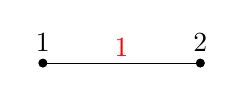
\begin{tikzpicture}[scale=1, every node/.style={circle, draw, fill=black, inner sep=1pt}]
      \node[label=above:{1}] (central) at (-2, 0) {};
      \node[label=above:{2}] (b1) at (0, 0) {};
      \draw (central) -- (b1) node[midway, above, text=red, fill=none, draw=none] {1};
    \end{tikzpicture}
    \caption{The unique $\alpha$-labeling of $B(1,1)$}
    \label{fig:rsf-banana-tree-1-1}
  \end{figure}
  Let $n > 1$ and let $f$ be a graceful labeling of a $B(n, 1)$ tree. Assume that $f(r) = x \in \{2, 3, \dots, n\}$. Then, there must exist vertices $a_i$ and $a_{i'}$ such that $f(a_i) = x - 1$ and $f(a_{i'}) = x + 1$. We compute
  $$
  f^*(r a_i) = |x - (x-1)| = 1 \quad \mbox{ and } \quad f^*(r a_{i'}) = |x - (x+1)| = 1,
  $$
  which is a contradiction since $f$ is graceful. Therefore, $f(r) \in \{1, n+1\}$. In the following table we give the two unique $\alpha$-labelings $f_1$ and $f_2$ of the $B(n,1)$ tree. Note that the labels of leaves $a_i$ are uniquely determined up to isomorphism, therefore there are no other $\alpha$-labelings of the $B(n,1)$ tree.
  $$
  \begin{array}{|c||c|c|}
    \hline
    & f_1 & f_2 = f_1^r  \\
    \hline \hline
    f_j(r) & 1 & n+1  \\
    \hline
    f_j(a_i) & i+1 & i  \\
    \hline \hline
    \alpha_j & 1 & n  \\
    \hline
  \end{array}
  $$

  \begin{figure}[H]
    \centering
    \begin{minipage}{0.4\textwidth}
      \centering
      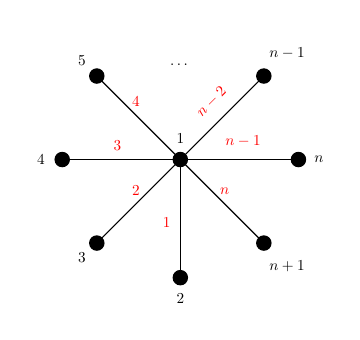
\begin{tikzpicture}[scale=0.75, every node/.style={circle, draw, fill=black, scale=0.55}, tight/.style={inner sep=0.02pt}]
        % Define the number of leaf vertices
        \def\n{7}
        % Define the radius for the leaf vertices
        \def\radius{2cm}

        % Draw the central vertex
        \node[circle, draw, fill=black, label=above:{$1$}] (C) at (0,0) {};

        % Draw the leaf vertices and connect them to the central vertex
        \foreach \i in {1,...,\n}
        {
          % Place each leaf vertex in a circular arrangement
          \coordinate (V\i) at ({135 + 360/(\n + 1) * (\i - 1)}:\radius) {};
          % Draw edge from central vertex to each leaf vertex
        }

        \node[circle, draw, fill=black, label=above left:{$5$}] at (V1) {};
        \node[circle, draw, fill=black, label=left:{$4$}] at (V2) {};
        \node[circle, draw, fill=black, label=below left:{$3$}] at (V3) {};
        \node[circle, draw, fill=black, label=below:{$2$}] at (V4) {};
        \node[circle, draw, fill=black, label=below right:{$n+1$}] at (V5) {};
        \node[circle, draw, fill=black, label=right:{$n$}] at (V6) {};
        \node[circle, draw, fill=black, label=above right:{$n-1$}] at (V7) {};

        \draw (C) -- (V1) node[midway, above, text=red, fill=none, draw=none] {$4$};
        \draw (C) -- (V2) node[midway, above, text=red, fill=none, draw=none] {$3$};
        \draw (C) -- (V3) node[midway, above, text=red, fill=none, draw=none] {$2$};
        \draw (C) -- (V4) node[midway, left, text=red, fill=none, draw=none] {$1$};
        \draw (C) -- (V5) node[midway, above, text=red, fill=none, draw=none] {$n$};
        \draw (C) -- (V6) node[tight, midway, above, text=red, fill=none, draw=none] {$n-1$};
        \draw (C) -- (V7) node[tight, midway, above, sloped, text=red, fill=none, draw=none] {$n-2$};

        \node[draw=none, fill=none] (dots) at (90:0.8*\radius) {\textbf{$\cdots$}};
      \end{tikzpicture}
      \caption*{$\alpha$-labeling $f_1$ of $B(n, 1)$} \label{fig:B(n,1)a}
    \end{minipage}
    \hspace{1cm}
    \begin{minipage}{0.4\textwidth}
      \centering
      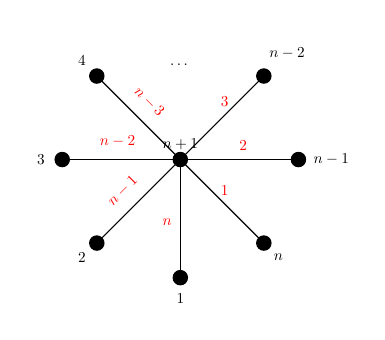
\begin{tikzpicture}[scale=0.75, every node/.style={circle, draw, fill=black, scale=0.55}, tight/.style={inner sep=0.02pt}]
        % Define the number of leaf vertices
        \def\n{7}
        % Define the radius for the leaf vertices
        \def\radius{2cm}

        % Draw the central vertex
        \node[circle, draw, fill=black] (C) at (0,0) {};
        \node[draw=none, fill=none, label={$n+1$}] at (0, -0.3) {};

        % Draw the leaf vertices and connect them to the central vertex
        \foreach \i in {1,...,\n}
        {
          % Place each leaf vertex in a circular arrangement
          \coordinate (V\i) at ({135 + 360/(\n + 1) * (\i - 1)}:\radius) {};
          % Draw edge from central vertex to each leaf vertex
        }

        \node[circle, draw, fill=black, label=above left:{$4$}] at (V1) {};
        \node[circle, draw, fill=black, label=left:{$3$}] at (V2) {};
        \node[circle, draw, fill=black, label=below left:{$2$}] at (V3) {};
        \node[circle, draw, fill=black, label=below:{$1$}] at (V4) {};
        \node[circle, draw, fill=black, label=below right:{$n$}] at (V5) {};
        \node[circle, draw, fill=black, label=right:{$n-1$}] at (V6) {};
        \node[circle, draw, fill=black, label=above right:{$n-2$}] at (V7) {};

        \draw (C) -- (V1) node[tight, midway, above, sloped, text=red, fill=none, draw=none] {$n-3$};
        \draw (C) -- (V2) node[tight, midway, above, text=red, fill=none, draw=none] {$n-2$};
        \draw (C) -- (V3) node[tight, midway, above, sloped, text=red, fill=none, draw=none] {$n-1$};
        \draw (C) -- (V4) node[midway, left, text=red, fill=none, draw=none] {$n$};
        \draw (C) -- (V5) node[midway, above, text=red, fill=none, draw=none] {$1$};
        \draw (C) -- (V6) node[midway, above, text=red, fill=none, draw=none] {$2$};
        \draw (C) -- (V7) node[midway, above, text=red, fill=none, draw=none] {$3$};

        \node[draw=none, fill=none] (dots) at (90:0.8*\radius) {\textbf{$\cdots$}};
      \end{tikzpicture}
      \caption*{$\alpha$-labeling $f_2$ of $B(n, 1)$} \label{fig:B(n,1)b}
    \end{minipage}
    \caption{Two $\alpha$-labelings of $B(n, 1)$} \label{fig:B(n,1)}
  \end{figure}

  The labeling $f_1$ is graceful because $f^*_1(r a_i) = |1 - (i + 1)| = i$ for all $i \in [n]$ and therefore $\mathcal{F}^*_1 = [n]$. We can see that $\alpha_1 = 1$ since $f_1(r) = 1$ and $f_1(a_1) = 2$. We can also see that $f_1(r) = 1 \leq 1 = \alpha_1 < i + 1 = f_1(a_i)$ for all $i \in [n]$. Therefore, $f_1$ is indeed an $\alpha$-labeling of the $B(n, 1)$ tree.

  The labeling $f_2$ is the complementary labeling of $f_1$ and therefore it is also an $\alpha$-labeling of the $B(n, 1)$ tree, with $\alpha_2 = \overline{\alpha_1} = n + 1 - \alpha_1 = n$.
\end{proof}

We note that $B(1,2) \cong P_3$ and $B(1,3) \cong P_4$. It was already shown in \cite{R67} that paths $P_n$ are $\alpha$-labelable. Here we give all their $\alpha$-labelings.

\begin{theorem}
  The $B(1, 2)$ tree and the $B(1, 3)$ tree are have exactly 2 distinct $\alpha$-labelings.
\end{theorem}

\begin{proof}
  There are 3 non-isomorphic labelings of the $B(1, 2)$ tree. The labeling $f_1$ of $B(1, 2)$ is shown in Figure \ref{fig:B(1,2)}. It is an $\alpha$-labeling with $\alpha_1 = 1$. The labeling $f_2$ of $B(1, 2)$ is the complementary labeling of $f_1$, so it is also an $\alpha$-labeling with $\alpha_2 = \overline{\alpha_1} = 3 - 1 = 2$.

  The only other non-isomorphic labeling of the $B(1, 2)$ tree is when the central vertex is labeled by $2$, however it is not even graceful.

  \begin{figure}[H]
    \centering
    \begin{minipage}{0.4\textwidth}
      \centering
      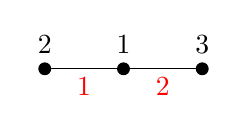
\begin{tikzpicture}[scale=0.5, every node/.style={circle, draw, fill=black, inner sep=1.5pt}]
        \node[label=above:{2}] (b1) at (-2, 0) {};

        \node[label=above:{1}] (central) at (0, 0) {};

        \node[label=above:{3}] (b2) at (2, 0) {};

        \draw (central) -- (b1) node[midway, below, text=red, fill=none, draw=none] {1};
        \draw (central) -- (b2) node[midway, below, text=red, fill=none, draw=none] {2};
      \end{tikzpicture}
      \caption*{$\alpha$-labeling $f_1$ of $B(1, 2)$} \label{fig:B(1,2)a}
    \end{minipage}
    \begin{minipage}{0.45\textwidth}
      \centering
      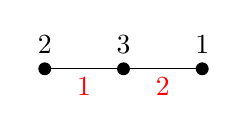
\begin{tikzpicture}[scale=0.5, every node/.style={circle, draw, fill=black, inner sep=1.5pt}]
        \node[label=above:{2}] (b1) at (-2, 0) {};

        \node[label=above:{3}] (central) at (0, 0) {};

        \node[label=above:{1}] (b2) at (2, 0) {};

        \draw (central) -- (b1) node[midway, below, text=red, fill=none, draw=none] {1};
        \draw (central) -- (b2) node[midway, below, text=red, fill=none, draw=none] {2};
      \end{tikzpicture}
      \caption*{$\alpha$-labeling $f_2$ of $B(1, 2)$} \label{fig:B(1,2)b}
    \end{minipage}
    \caption{Two $\alpha$-labelings of $B(1, 2)$}\label{fig:B(1,2)}
  \end{figure}

  There are $12$ non-isomorphic labelings of the $B(1, 3)$ tree. Only two of them, presented in Figure~\ref{fig:B(1,3)}, are $\alpha$-labelings. In the case of $f_1$, it is easy to see $\alpha_1 = 2$. The other labeling $f_2$ is the complementary labeling of $f_1$, with $\alpha_2 = \overline{\alpha_1} = 4 - 2 = 2$.
  \begin{figure}[H]
    \centering
    \begin{minipage}{0.4\textwidth}
      \centering
      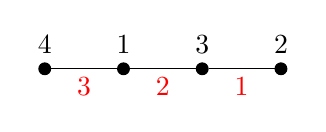
\begin{tikzpicture}[scale=0.5, every node/.style={circle, draw, fill=black, inner sep=1.5pt}]
        \node[label=above:{4}] (b1) at (-2, 0) {};

        \node[label=above:{1}] (central) at (0, 0) {};

        \node[label=above:{3}] (b2) at (2, 0) {};

        \node[label=above:{2}] (l11) at (4, 0) {};

        \draw (central) -- (b1) node[midway, below, text=red, fill=none, draw=none] {3};
        \draw (central) -- (b2) node[midway, below, text=red, fill=none, draw=none] {2};
        \draw (b2) -- (l11) node[midway, below, text=red, fill=none, draw=none] {1};
      \end{tikzpicture}
      \caption*{$\alpha$-labeling $f_1$ of $B(1, 3)$} \label{fig:B(1,3)a}
    \end{minipage}
    \hspace*{1cm}
    \begin{minipage}{0.4\textwidth}
      \centering
      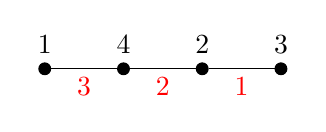
\begin{tikzpicture}[scale=0.5, every node/.style={circle, draw, fill=black, inner sep=1.5pt}]
        \node[label=above:{1}] (b1) at (-2, 0) {};

        \node[label=above:{4}] (central) at (0, 0) {};

        \node[label=above:{2}] (b2) at (2, 0) {};

        \node[label=above:{3}] (l11) at (4, 0) {};

        \draw (central) -- (b1) node[midway, below, text=red, fill=none, draw=none] {3};
        \draw (central) -- (b2) node[midway, below, text=red, fill=none, draw=none] {2};
        \draw (b2) -- (l11) node[midway, below, text=red, fill=none, draw=none] {1};
      \end{tikzpicture}
      \caption*{$\alpha$-labeling $f_2$ of $B(1, 3)$} \label{fig:B(1,3)b}
    \end{minipage}
    \caption{Two $\alpha$-labelings of $B(1, 3)$}\label{fig:B(1,3)}
  \end{figure}
\end{proof}

\begin{theorem}
  The $B(1, k)$ tree is $\alpha$-labelable for $k \geq 4$ and has exactly 4 distinct $\alpha$-labelings.
\end{theorem}

\begin{proof}
  By Theorem \ref{thm:principal-partition}, we know that we only need to find all the $\alpha$-labelings of the $B(1, k)$ tree when $f(r) = 1$. The four possible labelings for $B(1, k)$ are shown in the following table. Note that the values of $f(c_1)$, $f(r)$ and $f(a_1)$ uniquely determine the values of leaves of the induced star $S_k^1$.
  $$
  \begin{array}{|c||c|c|c|c|}
    \hline
    & f_1 & f_2 = f_1^r & f_3 = \overline{f_1} & f_4= \overline{f_1^r} \\
    \hline \hline
    f_i(r) & 2 & 1 & k & k+1 \\
    \hline
    f_i(a_1) & 3 & k+1 & k-1 & 1 \\
    \hline
    f_i(c_1) & 1 & 2 & k+1 & k \\
    \hline
    \mathcal{F}_i(L_1) & \{4, \ldots, k+1\} & \{3, \ldots, k\} & \{1, \ldots, k-2\} & \{2, \ldots, k-1\} \\
    \hline
    \alpha_i & 2 & 2 & k-1 & k-1 \\
    \hline
  \end{array}
  \label{tab:alpha-labelings}
  $$
  In the Figure \ref{fig:B(1,k)} we compute the values of $f^*$ to show that the four labelings are in fact $\alpha$-labelings.  We note that $\alpha_1 = 1$ for $f_1$ since $f_1(r) = 2$, $f(a_1) = 3$ and $f_1^*(r a_1) = |2-3|=1$. The labeling $f_2$ is the reverse of $f_1$ so it is also an $\alpha$-labeling of the $B(1,k)$ tree with $\alpha_2 = \alpha_1^r = 2$. The labeling $f_3$ is the complementary labeling of $f_1$ so it is also an $\alpha$-labeling of the $B(1,k)$ tree with $\alpha_3 = \overline{\alpha_1} = k - 1$. The labeling $f_4$ is the reverse of $f_3$ so it is also an $\alpha$-labeling of the $B(1,k)$ tree with $\alpha_4 = \alpha_3^r = k - 1$.

  \begin{figure}[H]
    \centering
    \begin{minipage}{0.4\textwidth}
      \centering
      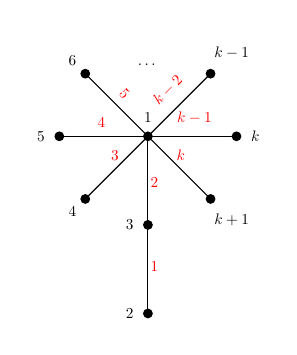
\begin{tikzpicture}[scale=0.75, every node/.style={circle, draw, fill=black, scale=0.55}, tight/.style={inner sep=0.02pt}]
        % Define the number of leaf vertices
        \def\n{7}
        % Define the radius for the leaf vertices
        \def\radius{1.5cm}

        % Draw the central vertex
        \node[circle, draw, fill=black, inner sep=2pt, label=above:1] (c) at (0,0) {};
        \node[circle, draw, fill=black, inner sep=2pt, label=left:2] (r) at (0,-3) {};

        % Draw the leaf vertices and connect them to the central vertex
        \foreach \i in {1,...,\n}
        {
          % Place each leaf vertex in a circular arrangement
          \coordinate (V\i) at ({135 + 360/(\n + 1) * (\i - 1)}:\radius) {};
          % Draw edge from central vertex to each leaf vertex
        }

        \node[circle, draw, fill=black, inner sep=2pt, label=above left:6] at (V1) {};
        \node[circle, draw, fill=black, inner sep=2pt, label=left:5] at (V2) {};
        \node[circle, draw, fill=black, inner sep=2pt, label=below left:4] at (V3) {};
        \node[circle, draw, fill=black, inner sep=2pt, label=left:3] at (V4) {};
        \node[circle, draw, fill=black, inner sep=2pt, label=below right:{$k+1$}] at (V5) {};
        \node[circle, draw, fill=black, inner sep=2pt, label=right:{$k$}] at (V6) {};
        \node[circle, draw, fill=black, inner sep=2pt, label=above right:{$k-1$}] at (V7) {};

        \draw (c) -- (V1) node[midway, above, sloped, text=red, fill=none, draw=none] {5};
        \draw (c) -- (V2) node[midway, above,  text=red, fill=none, draw=none] {4};
        \draw (c) -- (V3) node[midway, above, text=red, fill=none, draw=none] {3};
        \draw (c) -- (V4) node[tight, midway, above, text=red, right, fill=none, draw=none] {2};
        \draw (c) -- (V5) node[midway, above, text=red, fill=none, draw=none] {$k$};
        \draw (c) -- (V6) node[tight, midway, above, text=red, fill=none, draw=none] {$k-1$};
        \draw (c) -- (V7) node[tight, midway, above, sloped, text=red, fill=none, draw=none] {$k-2$};

        \draw (V4) -- (r) node[tight, midway, right, text=red, fill=none, draw=none] {1};

        \node[draw=none, fill=none] (dots) at (90:0.8*\radius) {\textbf{$\cdots$}};
      \end{tikzpicture}

      \caption*{$\alpha$-labeling $f_1$ with $\alpha_1 = 2$} \label{fig:B(1,k)a}
    \end{minipage}
    \hspace*{1cm}
    \begin{minipage}{0.4\textwidth}
      \centering
      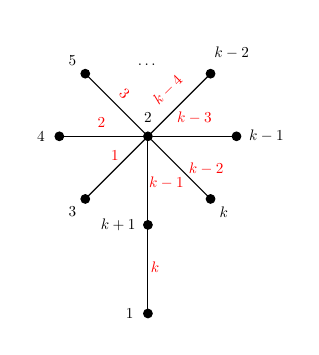
\begin{tikzpicture}[scale=0.75, every node/.style={circle, draw, fill=black, scale=0.55}, tight/.style={inner sep=0.02pt}]
        % Define the number of leaf vertices
        \def\n{7}
        % Define the radius for the leaf vertices
        \def\radius{1.5cm}

        % Draw the central vertex
        \node[circle, draw, fill=black, inner sep=2pt, label=above:2] (c) at (0,0) {};
        \node[circle, draw, fill=black, inner sep=2pt, label=left:1] (r) at (0,-3) {};

        % Draw the leaf vertices and connect them to the central vertex
        \foreach \i in {1,...,\n}
        {
          % Place each leaf vertex in a circular arrangement
          \coordinate (V\i) at ({135 + 360/(\n + 1) * (\i - 1)}:\radius) {};
          % Draw edge from central vertex to each leaf vertex
        }

        \node[circle, draw, fill=black, inner sep=2pt, label=above left:5] at (V1) {};
        \node[circle, draw, fill=black, inner sep=2pt, label=left:4] at (V2) {};
        \node[circle, draw, fill=black, inner sep=2pt, label=below left:3] at (V3) {};
        \node[circle, draw, fill=black, inner sep=2pt, label=left:{$k+1$}] at (V4) {};
        \node[circle, draw, fill=black, inner sep=2pt, label=below right:{$k$}] at (V5) {};
        \node[circle, draw, fill=black, inner sep=2pt, label=right:{$k-1$}] at (V6) {};
        \node[circle, draw, fill=black, inner sep=2pt, label=above right:{$k-2$}] at (V7) {};

        \draw (c) -- (V1) node[midway, above, sloped, text=red, fill=none, draw=none] {3};
        \draw (c) -- (V2) node[midway, above, text=red, fill=none, draw=none] {2};
        \draw (c) -- (V3) node[midway, above, text=red, fill=none, draw=none] {1};
        \draw (c) -- (V4) node[tight, midway, right, text=red, fill=none, draw=none] {$k-1$};
        \draw (c) -- (V5) node[midway, right, text=red, fill=none, draw=none] {$k-2$};
        \draw (c) -- (V6) node[tight, midway, above,  text=red, fill=none, draw=none] {$k-3$};
        \draw (c) -- (V7) node[tight, midway, above, sloped, text=red, fill=none, draw=none] {$k-4$};

        \draw (V4) -- (r) node[tight, midway, right, text=red, fill=none, draw=none] {$k$};

        \node[draw=none, fill=none] (dots) at (90:0.8*\radius) {\textbf{$\cdots$}};
      \end{tikzpicture}

      \caption*{$\alpha$-labeling $f_2$ with $\alpha_2 = 2$} \label{fig:B(1,k)b}
    \end{minipage}
    \begin{minipage}{0.4\textwidth}
      \centering
      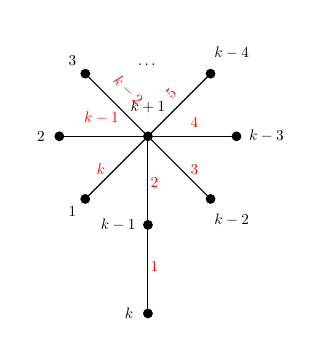
\begin{tikzpicture}[scale=0.75, every node/.style={circle, draw, fill=black, scale=0.55}, tight/.style={inner sep=0.02pt}]
        % Define the number of leaf vertices
        \def\n{7}
        % Define the radius for the leaf vertices
        \def\radius{1.5cm}

        % Draw the central vertex
        \node[circle, draw, fill=black, inner sep=2pt, label=above:{$k+1$}] (c) at (0,0) {};
        \node[circle, draw, fill=black, inner sep=2pt, label=left:{$k$}] (r) at (0,-3) {};

        % Draw the leaf vertices and connect them to the central vertex
        \foreach \i in {1,...,\n}
        {
          % Place each leaf vertex in a circular arrangement
          \coordinate (V\i) at ({135 + 360/(\n + 1) * (\i - 1)}:\radius) {};
          % Draw edge from central vertex to each leaf vertex
        }

        \node[circle, draw, fill=black, inner sep=2pt, label=above left:3] at (V1) {};
        \node[circle, draw, fill=black, inner sep=2pt, label=left:2] at (V2) {};
        \node[circle, draw, fill=black, inner sep=2pt, label=below left:1] at (V3) {};
        \node[circle, draw, fill=black, inner sep=2pt, label=left:{$k-1$}] at (V4) {};
        \node[circle, draw, fill=black, inner sep=2pt, label=below right:{$k-2$}] at (V5) {};
        \node[circle, draw, fill=black, inner sep=2pt, label=right:{$k-3$}] at (V6) {};
        \node[circle, draw, fill=black, inner sep=2pt, label=above right:{$k-4$}] at (V7) {};

        \draw (c) -- (V1) node[tight, midway, above, sloped, text=red, fill=none, draw=none] {$k-2$};
        \draw (c) -- (V2) node[tight, midway, above, text=red, fill=none, draw=none] {$k-1$};
        \draw (c) -- (V3) node[midway, left, text=red, fill=none, draw=none] {$k$};
        \draw (c) -- (V4) node[tight, midway, right, text=red, fill=none, draw=none] {2};
        \draw (c) -- (V5) node[midway, right, text=red, fill=none, draw=none] {3};
        \draw (c) -- (V6) node[midway, above, text=red, fill=none, draw=none] {4};
        \draw (c) -- (V7) node[midway, above, sloped, text=red, fill=none, draw=none] {5};

        \draw (V4) -- (r) node[tight, midway, right, text=red, fill=none, draw=none] {1};

        \node[draw=none, fill=none] (dots) at (90:0.8*\radius) {\textbf{$\cdots$}};
      \end{tikzpicture}
      \caption*{$\alpha$-labeling $f_3$ with $\alpha_3 = k - 1$} \label{fig:B(1,k)c}
    \end{minipage}
    \hspace*{1cm}
    \begin{minipage}{0.4\textwidth}
      \centering
      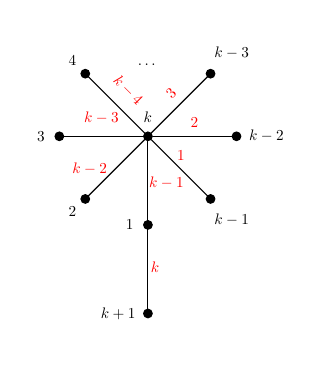
\begin{tikzpicture}[scale=0.75, every node/.style={circle, draw, fill=black, scale=0.55}, tight/.style={inner sep=0.02pt}]
        % Define the number of leaf vertices
        \def\n{7}
        % Define the radius for the leaf vertices
        \def\radius{1.5cm}

        % Draw the central vertex
        \node[circle, draw, fill=black, inner sep=2pt, label=above:{$k$}] (c) at (0,0) {};
        \node[circle, draw, fill=black, inner sep=2pt, label=left:{$k+1$}] (r) at (0,-3) {};

        % Draw the leaf vertices and connect them to the central vertex
        \foreach \i in {1,...,\n}
        {
          % Place each leaf vertex in a circular arrangement
          \coordinate (V\i) at ({135 + 360/(\n + 1) * (\i - 1)}:\radius) {};
          % Draw edge from central vertex to each leaf vertex
        }

        \node[circle, draw, fill=black, inner sep=2pt, label=above left:4] at (V1) {};
        \node[circle, draw, fill=black, inner sep=2pt, label=left:3] at (V2) {};
        \node[circle, draw, fill=black, inner sep=2pt, label=below left:2] at (V3) {};
        \node[circle, draw, fill=black, inner sep=2pt, label=left:{1}] at (V4) {};
        \node[circle, draw, fill=black, inner sep=2pt, label=below right:{$k-1$}] at (V5) {};
        \node[circle, draw, fill=black, inner sep=2pt, label=right:{$k-2$}] at (V6) {};
        \node[circle, draw, fill=black, inner sep=2pt, label=above right:{$k-3$}] at (V7) {};

        \draw (c) -- (V1) node[tight, midway, above, sloped, text=red, fill=none, draw=none] {$k-4$};
        \draw (c) -- (V2) node[tight, midway, above, text=red, fill=none, draw=none,] {$k-3$};
        \draw (c) -- (V3) node[midway, left, text=red, fill=none, draw=none] {$k-2$};
        \draw (c) -- (V4) node[tight, midway, right, text=red, fill=none, draw=none] {$k-1$};
        \draw (c) -- (V5) node[midway, above, text=red, fill=none, draw=none] {1};
        \draw (c) -- (V6) node[midway, above, text=red, fill=none, draw=none] {2};
        \draw (c) -- (V7) node[midway, above, sloped, text=red, fill=none, draw=none] {3};

        \draw (V4) -- (r) node[tight, midway, right, text=red, fill=none, draw=none] {$k$};

        \node[draw=none, fill=none] (dots) at (90:0.8*\radius) {\textbf{$\cdots$}};
      \end{tikzpicture}

      \caption*{$\alpha$-labeling $f_4$ with $\alpha_4 = k - 1$} \label{fig:B(1,k)d}
    \end{minipage}
    \caption{Four possible $\alpha$-labelings of $B(1, k)$} \label{fig:B(1,k)}
  \end{figure}

  We only need to show that the value of $f(a_1)$ is uniquely determined when $f(r) = 1$ and $f(c_1) = 2$. Suppose $f(a_1) \neq k + 1$, i.e. $3 \le f(a_1) \le k$. Then, we would have $f^*(r a_1) = f(a_1) - 1 \le k - 1$ and $f(c_1 a_1) = f(a_1) - 2 \le k - 2$. Now, we need to have $f^*(c_1 v) = k$ for some $v \in \mathcal{L}_1$ for the labeling to be graceful. But this is not possible since $f(c_1) = 2$ and $f(v) \le k + 1$, so we would have $f^*(c_1 v) = f(v) - 2 \le k - 1$. This is a contradiction, so we must have $f(a_1) = k + 1$.
\end{proof}

\begin{theorem}
  \label{thm:A_1(2,k)}
  $$
  \mathcal{A}_1(2, k) =
  \begin{cases}
    \emptyset,& k = 2\\
    \{f\},& k \ge 3
  \end{cases}
  $$
  where
  $$
  \begin{array}{lcl}
    f(r) & = & 1 \\
    f(c_i) & = & i + 1 \\
    f(a_i) & = & (3 - i)k + 1 \\
    \mathcal{F}(\mathcal{L}_1) & = & \{k + 3, k + 4, \dots, 2k\}\\
    \mathcal{F}(\mathcal{L}_2) & = & \{4, 5, \dots, k-1, k, k+2\}\\
  \end{array}
  $$
\end{theorem}

\begin{proof}
  Let $k = 2$. Then, by definition, a putative $\alpha$-labeling $f \in \mathcal{A}_1(2,2)$ must have $f(r) = 1$ and without loss of generality, we can set $f(c_1) = 2$, $f(c_3) = 3$. We have two cases: $f(a_1) = 4$ and $f(a_1) = 5$. If $f(a_1) = 4$, we have $f(a_2) = 5$, but then $f^*(a_1 c_1) = 4 - 2 = 2 = 5 - 3 = f^*(a_2 c_2)$ so $f$ is not even graceful. If we have $f(a_1) = 5$, then we have $f(a_1 c_1) = 5 - 2 = 3 = 4 - 1 = f^*(r a_2)$ so $f$ is not even graceful. Therefore, $\mathcal{A}_1(2, 2) = \emptyset$.

  Let $k \ge 3$. Then, by definition, a putative $\alpha$-labeling $f \in \mathcal{A}_1(2,2)$ must have $f(r) = 1$ and without loss of generality, we can set $f(c_1) = 2$, $f(c_3) = 3$.

  We know that we must have $f^*(vw) = 2k$ for some $vw \in E(B(2,k))$. This is only possible for $r a_1$ and $r a_2$.

  Suppose $f^*(r a_2) = 2k$, i.e. $f(a_2) = 2 k + 1$ and $f^*(a_2 c_2) = 2k - 2$. Then, we would need to have $f^*(vw) = 2k - 1$. This can't be $r a_1$, since if $f^*(r a_1) = 2k - 1$, then we would have $f(a_1) = 2k$ and $f^*(a_1 c_1) = 2k - 2$, but then $f$ wouldn't even be graceful. If $f^*(v c_1) = 2k -1$, then we would have $f(v) = 2k + 1$, which is not possible. If $f^*(v c_2) = 2k - 1$, then we would have $f(v) = 2k + 2$, but that is also not possible. Therefore, we must have $f(a_1) = 2k + 1$.

  Then, we must have $f^*(v c_i) = 2k - 2$ for some $i \in \{1,2\}$. If, $i = 2$, we have $f(v) = f(c_2) + 2k - 2 = 2k + 1$, but that is not possible since $f(a_1) = 2k + 1$. Inductively, we can show that $\mathcal{F}(\mathcal{L}_1) = \{2k, 2k - 1, \dots, k + 3\}$.

  Now we need to have $f^*(r a_2) = k$ or $f^*(a_2 c_2) = k$. If we have $f^*(a_2 c_2) = k$, we would have $f(a_2) = k + 3$, but $k + 3 \in \mathcal{F}(\mathcal{L}_1)$, so we must have $f^*(r a_2) = k$, i.e. $f(a_2) = k + 2$. The labes that we haven't yet assigned to any vertex are $\{4, 5, \dots, k-1, k, k+2\}$, so we must have $\mathcal{F}(\mathcal{L}_2) = \{4, 5, \dots, k-1, k, k+2\}$. This is the only possible labeling of the $B(2,k)$ tree with $f(r) = 1$, and it is exactly the labeling $f$.
\end{proof}

\begin{theorem}
  \label{thm:A_2(2,k)}
  For any $k \ge 2$, we have
  $$
  \mathcal{A}_2(2, k) = \{f_y \mid k + 3 \le y \le 2k + 1\},
  $$
  where
  $$
  \begin{array}{lcl}
    f_y(r) & = & 2 \\
    f_y(c_1) & = & 1 \\
    f_y(c_2) & = & 3 \\
    f_y(a_1) & = & y \\
    f_y(a_2) & = & 2k + 5 - y \\
    \mathcal{F}_y(\mathcal{L}_1) & = & \{y + 1, y + 2, \dots, 2k + 1\} \cup \{y - 2i \mid 1 \le i \le y - k - 3\}\\
    \mathcal{F}_y(\mathcal{L}_2) & = & \left( \{4, 5, \dots, 2k + 4 - y\} \cup \{2k + 5 - y + 2i \mid 1 \le i \le y - k - 3\} \right)\\
  \end{array}
  $$
\end{theorem}

\begin{proof}
  Firstly, we will show that $\{f_y \mid k + 3 \le y \le 2k + 1\} \subseteq \mathcal{A}_2(2, k)$, i.e. that all the $f_y$ are $\alpha$-labelings of $B(2, k)$. Then we will show that $\mathcal{A}_2(2, k) \subseteq \{f_y \mid k + 3 \le y \le 2k + 1\}$, i.e. that all the $\alpha$-labelings of $B(2,k)$ with $f(r) = 2$ are exactly $f_y$ for $k + 3 \le y \le 2k + 1$.

  \begin{enumerate}
    \item We need to show $\mathcal{F} = [2n + 1]$. We can see that $\mathcal{F}(RC) = [3]$. Therefore, we need to show
      $$
      \mathcal{F}\left(\mathcal{B}_1 \cup \mathcal{B}_2\right) = \{4,5,\dots,2k+1\}
      $$

      We know that
      \begin{align*}
        \mathcal{F}(\mathcal{B}_1) &= \{y + 1, \dots, 2k + 1\} \cup \{y - 2(y - k - 3), y - 2(y - k - 4), \dots, y\}\\
        &= \{y + 1, \dots, 2k + 1\} \cup \{2k + 6 - y, 2k + 8 - y, \dots, y\}
      \end{align*}
      and
      \begin{align*}
        \mathcal{F}(\mathcal{B}_2) &= \{4, \dots, 2k + 5 - y\} \cup \{2k + 5 - y + 2, \dots, 2k + 5 - y + 2(y - k - 3)\}\\
        &= \{4, 5, \dots, 2k + 5 - y\} \cup \{2k + 7 - y, 2k + 9 - y, \dots, y - 1\}
      \end{align*}
      Now, we can see that
      \begin{align*}
        \mathcal{F}\left(\mathcal{B}_1 \cup \mathcal{B}_2\right) &= \mathcal{F}(\mathcal{B}_1) \cup \mathcal{F}(\mathcal{B}_2)\\
        &= \{y + 1, \dots, 2k + 1\} \cup \{2k + 6 - y, 2k + 8 - y, \dots, y\} \\ &\quad\;\cup \{4, 5, \dots, 2k + 5 - y\} \cup \{2k + 7 - y, 2k + 9 - y, \dots, y - 1\}\\
        &= \{4, 5, \dots, 2k + 5 - y\} \cup \{2k + 6 - y, \dots, y\} \cup \{y + 1, \dots, 2k + 1\}\\
        &= \{4, 5, \dots, 2k + 1\}
      \end{align*}

      Secondly, we need to show $\mathcal{F}^* = [2k]$.

      We know that

      \begin{align*}
        \mathcal{F}^*(\mathcal{B}_1) &= \{y + 1 - 1, \dots, 2k + 1 - 1\} \cup \{2k + 6 - y - 1, \dots, y - 1\} \\
        &= \{y, \dots, 2k\} \cup \{2k + 5 - y, 2k + 7 - y, \dots, y - 1\},
      \end{align*}
      \begin{align*}
        \mathcal{F}^*(\mathcal{B}_2) &= \{4 - 3, 5 - 3, \dots, 2k + 5 - y - 3\} \cup \{2k + 7 - y - 3, \dots, y - 1 - 3\} \\
        &= \{1, 2, \dots, 2k + 2 - y\} \cup \{2k + 4 - y, 2k + 6 - y, \dots, y - 4\}
      \end{align*}
      and also, $f^*(r a_1) = y - 2$ and $f^*(r a_1) = 2k + 3 - y$. Thus, we have
      \begin{align*}
        \mathcal{F}^* &= \{y, \dots, 2k\} \cup \{2k + 5 - y, \dots, y - 1\} \cup \{1, 2, \dots, 2k + 2 - y\}\\ &\quad\;\cup \{2k + 4 - y, 2k + 6 - y, \dots, y - 4\} \cup \{y - 2, 2k + 3 - y\}\\
        &= \{y, \dots, 2k\} \cup \{2k + 3 - y, \dots, y - 1\} \cup \{1, 2, \dots, 2k + 2 - y\}\\ &\quad\;\cup \{2k + 4 - y, 2k + 6 - y, \dots, y - 2\} \\
        &= \{y, \dots, 2k\} \cup \{2k + 3 - y, 2k + 4 - y \dots, y - 1\} \cup \{1, 2, \dots, 2k + 2 - y\} \\
        &= \{1, 2, \dots, 2k\} = [2k]
      \end{align*}
      Finally, we know that the $\alpha$ inequality holds since $f(c_i) \le 3 < f(v)$ for all $v \in \mathcal{B}_i$ and $i = 1,2$, as well as $f(r) = 2 \le 3 < f(a_i)$ for $i = 1,2$. Thus, we have shown $\{f_y \mid k + 3 \le y \le 2k + 1\} \subseteq \mathcal{A}_2(2, k)$.

    \item Let $f \in \mathcal{A}_2(2,k)$ be an $\alpha$-labeling of $B(2,k)$ with $f(r)$. Then we know that, without loss of generality, we have $f(c_1) = 1$ and $f(c_2) = 3$, and we also know that $4 \in \mathcal{F}(\mathcal{B}_2)$ since $\alpha = 3$ and $2k + 1 \in \mathcal{F}(\mathcal{B}_1)$ since we need $2k \in \mathcal{F}^*$.

      Let $f(a_1) = x$ for some $x \in \{5, \dots, 2k\}$. Then we know $f(ra_1) = x - 2$ and $f^*(a_1 c_1) = x - 1$. Now, we know that $f(v) \neq x + 1$ for all $v \in \mathcal{B}_2$, since if it were, we would have $f^*(v c_2) = x + 1 - 3 = x - 2$, but then the labeling wouldn't even be graceful. Furthermore, we can inductively reason that $\{x, x+1, \dots, 2k + 1\} \subseteq \mathcal{F}(\mathcal{B}_1)$. This means that
      \begin{align*}
        |\{x, x+1, \dots 2k + 1\}| &\le |\mathcal{F}(\mathcal{B}_1)| \\
        2k + 1 - x + 1 &\le k - 1 \\
        2k + 3 - x &\le k \\
        x &\ge k + 3
      \end{align*}
      Now we have $\{x-1,x,x+1,\dots,2k\} \subseteq \mathcal{F}^*(\mathcal{B}_1)$ and $f^*(r a_1) = x - 2$. We also have $x - 1 \notin \mathcal{F}(\mathcal{B}_1)$, since we have $f^*(ra_1) = x - 2$ and $f$ wouldn't even be graceful. Therefore, $x - 1 \in \mathcal{F}(\mathcal{B}_2)$.

      Let $f(a_2) = z$. Then we have $f^*(r a_2) = z - 2$ and $f^*(a_2 c_2) = z - 3$. Now we know that $f(v) \neq z - 1$ for all $v \in \mathcal{B}_1$, since if it were, we would have $f^*(v c_1) = z - 1 - 1 = z - 2$, but then the labeling wouldn't even be graceful. Furthermore, we can inductively reason that $\{z, z-1, \dots, 4\} \subseteq \mathcal{F}(\mathcal{B}_1)$. This means that
      \begin{align*}
        |\{z, z-1, \dots, 4\}| &\le |\mathcal{F}(\mathcal{B}_1)| \\
        z - 4 + 1 &\le k - 1 \\
        z &\le k + 2
      \end{align*}
      Now we have $\{z - 3 , z - 4, \dots, 1\} \subseteq \mathcal{F}(\mathcal{B}_2)$. Furthermore, we know that $z + 1 \in \mathcal{F}(\mathcal{B}_1)$ since, otherwise we would have $f^*(v c_2) = z + 1 - 3 = z - 2 = f^*(r a_2)$ for some $v \in \mathcal{B}_2$ and the labeling wouldn't even be graceful. Now, we know that $z + 2 \in \mathcal{F}(\mathcal{B}_2)$ because we need to have $z - 1 \in \mathcal{F}^*$. Furthermore, we can inductively reason that $\{z + 1, z + 3, \dots, z + 2t - 1\} \subseteq \mathcal{F}(\mathcal{B}_1)$ for some $t \ge 0$ as well as $\{z + 2, z + 4, \dots, z + 2u\} \subseteq \mathcal{F}(\mathcal{B}_2)$ for some $u \ge 0$. Then, we have $\mathcal{F}(\mathcal{B}_1) = \{x, x + 1, \dots, 2k + 1\} \cup \{z + 1, z + 3, z + 2t - 1\}$, i.e.
      \begin{align*}
        k - 1 &= |\{x, x + 1, \dots, 2k + 1\}| + |\{z + 1, z + 3, z + 2t - 1\}| \\
        k - 1 &= (2k + 1 - x + 1) + t \\
        0 &= k + 3 - x + t\\
        t &= x - k - 3
      \end{align*}
      Let's look at the vertex $v$ with the label $x - 1$. We know it can't be in $\mathcal{B}_1$ since then we would have $f^*(v c_1) = x - 2 = f^*(r a_1)$. Therefore, we must have $x - 1 \in \mathcal{F}(\mathcal{B}_2)$. Now we need to find the edge with the induced label $x - 3$. This can only be $w c_1$ for some $w \in \mathcal{B}_1$. Furthermore, we can inductively reason that $\{x - 1, x - 3, \dots, x - 2t' + 1\} \in \mathcal{F}(\mathcal{B}_2)$ and $\{x - 2, x -  4, \dots, x - 2u'\} \in \mathcal{F}(\mathcal{B}_1)$  for sume $t', u' \ge 0$. We now know
      \begin{align*}
        z + 2t - 1 &= x - 2\\
        z + 2(x - k - 3) + 1 &= x \\
        z = 2k + 5 - x
      \end{align*}
      since $\{z + 1, z + 3, z + 2t - 1\} = \{x - 2, x -  4, \dots, x - 2u'\}$. Thus we have that $f$ is exactly $f_x$ from the set $\{f_y \mid k + 3 \le y \le 2k + 1\}$, i.e. $\mathcal{A}_2(2, k) \subseteq \{f_y \mid k + 3 \le y \le 2k + 1\}$.
  \end{enumerate}
  Thus, we have $\mathcal{A}_2(2, k) = \{f_y \mid k + 3 \le y \le 2k + 1\}$.
\end{proof}

\begin{corollary}
  $$
  A(2, k) =
  \begin{cases}
    2, & k = 1, 2\\
    2(k + 1),& k \ge 3
  \end{cases}
  $$
\end{corollary}

\begin{proof}
  We will look at three different cases: $k = 1$, $k = 2$ and $k \ge 3$.

  \begin{enumerate}
    \item Let $k = 1$. By Theorem \ref{thm:B(n,1)}, we know that $A(2, 1) = 2$.

    \item Let $k = 2$. From the Theorems \ref{thm:A_1(2,k)} and \ref{thm:A_2(2,k)}, we can see that $P(2, 2) = A_1(2,2) + A_2(2,2) = 0 + (2 \cdot 2 + 1 - (2 + 3) + 1) = 1$ and $C(2, 2) = A_2(2,2) = 1$. Therefore, by Theorem \ref{thm:A(n,k)_sum} we have that $A(2,2) = 4P(2,2) - 2C(2,2) = 4 - 2 = 2$.

    \item Let $k \ge 3$. From the Theorems \ref{thm:A_1(2,k)} and \ref{thm:A_2(2,k)}, we can see that $P(2, k) = A_1(2,k) + A_2(2,k) = 1 + (2k + 1 - (k + 3) + 1) = 1 + k - 1 = k$ and $C(2, k) = A_2(2,k) = (2k + 1 - (k + 3) + 1) = k - 1$. Therefore, by Theorem \ref{thm:A(n,k)_sum} we have that $A(2,k) = 4P(2,k) - 2C(2,k) = 4k - 2(k - 1) = 2k + 2 = 2(k + 1)$.
  \end{enumerate}
\end{proof}

The construction in the following theorem is inspired by the construction of the graceful labeling of superstar trees in \cite{MMK14}. Our result differs from theirs in the fact that we proved that this labeling is an $\alpha$-labeling, while in \cite{MMK14} it is only proven that it is a graceful labeling. Also, we are only looking at banana trees, not superstar trees. The labeling given by this construction is also the reverse labeling of the labeling given by the construction in \cite{SSS23}.

\begin{theorem}
  The $B(n, k)$ tree is $\alpha$-labelable for all $n \geq 3$ and $k > n$.
\end{theorem}

\begin{proof}
  The $B(n,k)$ tree has $[nk + 1]$ vertices. We define a labeling $f: V(B(n, k)) \rightarrow \mathbb{N}$
  (Figure \ref{fig:B(n,k)}) as follows:
  $$
  \begin{array}{lcl}
    f(r) & = & n + 1 \\
    f(c_i) & = & i \\
    f(a_i) & = & nk + (1-k)i + (n+2-i) \\
    \mathcal{F}(\mathcal{L}_i) & = & \{ nk + (1-k)i + 2, \ldots , nk + (1 - k)i + k\} \setminus \{f(a_i)\},
  \end{array}
  $$
  where $i = 1, \ldots, n$.

  First, we show that each vertex of the $B(n, k)$ tree is labeled by the distinct element of $[nk + 1]$.
  Obviously, vertices $c_1, \ldots, c_n, r$ are labeled by a distinct elements of $[n + 1]$. Now we discuss the lables of all other vertices, that is, we deterimine  $\mathcal{F}(\mathcal{B}) =  \mathcal{F}(\mathcal{B}_1) \cup \cdots \cup \mathcal{F}(\mathcal{B}_n)$, where $\mathcal{B}_i = \{a_i\} \cup \mathcal{L}_i = \{a_i,  l_{i,1}, \ldots, l_{i, k-2}\}$.
  Note that for the vertex $a_i$, $i \in [n]$, it holds that
  $$
  nk + (1-k)i + 2 - f(a_i)  = i-n-2 \le 0
  $$
  and
  $$
  nk + (1 - k)i + k - f(a_i) = k - n -2 + i \ge 0,
  $$
  since $k > n $. Therefore, the vertices of $\mathcal{B}_i$ are labeled by the distinct elements of
  $$
  \mathcal{F}(\mathcal{B}_i) = \{ nk + (1-k)i + 2, \dots, nk + (1-k)i + k\}.
  $$
  We also have that $\mathcal{F}(\mathcal{B}_i) \cap \mathcal{F}(\mathcal{B}_{i + 1}) = \emptyset$ since
  \begin{equation}\label{lab_bi}
    \mathcal{F}(\mathcal{B}_{i + 1}) = \{nk + (1-k)i +3 - k, \dots, nk + (1-k)i +1\}
  \end{equation}
  and
  $$
  \min{\mathcal{F}(\mathcal{B}_{i})} - \max{\mathcal{F}(\mathcal{B}_{i + 1})} = (nk + (1-k)i + 2) - ( nk + (1-k)i +1) = 1.
  $$

  \begin{figure}[H]
    \centering
    \begin{adjustbox}{max width=1.1\textwidth,center}
      \begin{tikzpicture}[scale=1.5, every node/.style={circle, draw, fill=black, inner sep=1.5pt, font=\footnotesize}]

        \node[label=below:{$ n + 1$}] (central) at (0, -2) {};

        \def\k{6} % Number of leaves in each star graph
        \def\leafradius{0.8} % Radius of the circular arrangement of leaves

        \node[label=above:{$1$}] (b1) at (-1.8, 0) {};
        \node[label=above:{$i$}] (b2) at (0, 2.3) {};
        \node[label=above:{$n$}] (b3) at (1.8, 0) {};

        \foreach \j in {1,...,\k} {
          \pgfmathsetmacro\leafangle{-90 - 360/\k * (\j-1)}

          \coordinate (l1\j) at ($(b1) + (\leafangle:\leafradius)$);
          \coordinate (l2\j) at ($(b2) + (\leafangle:\leafradius)$);
          \coordinate (l3\j) at ($(b3) + (\leafangle:\leafradius)$);
        }

        \node[label=right:{$nk -k + n + 2$}] at (l11) {};
        \node[label=left:{$nk - k + 3$}] at (l12) {};
        \node[label=left:{$nk - k + 4$}] at (l13) {};
        \node[label=right:{$nk$}] at (l15) {};
        \node[label=right:{$nk + 1$}] at (l16) {};

        \draw (b1) -- (l11);
        \draw (b1) -- (l12);
        \draw (b1) -- (l13);
        \draw (b1) -- (l15);
        \draw (b1) -- (l16);

        \node[label=right:{$nk + (1-k)i + n + 2 -i $}] at (l21) {};
        \node[label=left:{$nk + (1-k)i +2$}] at (l22) {};
        \node[label=left:{$nk + (1-k)i + 3$}] at (l23) {};
        \node[label=right:{$nk + (1-k)i + k - 1$}] at (l25) {};
        \node[label=right:{$nk + (1-k)i + k$}] at (l26) {};

        \draw (b2) -- (l21);
        \draw (b2) -- (l22);
        \draw (b2) -- (l23);
        \draw (b2) -- (l25);
        \draw (b2) -- (l26);

        \node[label=right:{$n + 2$}] at (l31) {};
        \node[label=left:{$n + 3$}] at (l32) {};
        \node[label=left:{$n + 4$}] at (l33) {};
        \node[label=right:{$n + k - 1$}] at (l35) {};
        \node[label=right:{$n + k$}] at (l36) {};

        \draw (b3) -- (l31);
        \draw (b3) -- (l32);
        \draw (b3) -- (l33);
        \draw (b3) -- (l35);
        \draw (b3) -- (l36);

        \foreach \j in {1,...,3} {
          \pgfmathsetmacro\dotangle{90}
          \node[draw=none, fill=none] at ($(b\j) + (\dotangle:0.75*\leafradius)$) {\textbf{$\cdots$}};
        }

        \draw (central) -- (l11);
        \draw (central) -- (l21);
        \draw (central) -- (l31);

        % \def\nlines{12}
        % \def\startingx{-2}
        % \foreach \i in {1,...,\nlines} {
        %   \draw (central) -- ({(\i-1) * (-2*\startingx)/(\nlines-1) + \startingx}, {-1.5 + abs(\i-(\nlines+1)/2)*0.05});
        % }

        % Optional: add dots to indicate missing parts in the middle
        \node[draw=none,fill=none] at (-2.4,1.2) {\huge{\reflectbox{$\ddots$}}};
        \node[draw=none,fill=none] at (2.45,1.2) {\huge{$\ddots$}};
        \node[draw=none, fill=none] at ($(b1) + (180:2.5*\leafradius)$) {\Large \textbf{$S^1_k$}};
        \node[draw=none, fill=none] at ($(b2) + (90:1.8*\leafradius)$) {\Large \textbf{$S^i_k$}};
        \node[draw=none, fill=none] at ($(b3) + (0:2.3*\leafradius)$) {\Large \textbf{$S^n_k$}};

      \end{tikzpicture}
    \end{adjustbox}
    \caption{The labeling $f$ of the  $B(n, k)$ tree}
    \label{fig:B(n,k)}
  \end{figure}
  Therefore,
  \begin{equation}\label{lab_b}
    \begin{array}{lcl}
      \mathcal{F}(\mathcal{B}) & = & \mathcal{F}(\mathcal{B}_n) \cup \cdots \cup \mathcal{F}(\mathcal{B}_{1}) = \\ & = &
      \{n+2, \ldots n+k\} \cup \cdots \cup \{nk-k+3, \ldots , nk+1\} = \\
      & = & \{ n + 2, n + 3, \dots, nk + 1\},\\
    \end{array}
  \end{equation}
  and we conclude that the vertices of the $B(n,k)$ tree are labeled with distinct elements of $[nk + 1]$.

  Now we show that the labeling $f$ is graceful. The edges of $S_k^i$, $i \in [n]$, are $E(S_k^i) = \{c_i a_i$, $c_i l_{i,1}, \ldots, c_i l_{i, k-2}\}$. Since $f(c_i) = i$ and the vertices of $\mathcal{B}_i$ are labeled by distinct elements of (\ref{lab_bi}) we have that
  $$
  \mathcal{F}^*(E(S_k^i)) = \{ f^*(c_i v) = |f(c_i) - f(v)| \, : \, v \in \mathcal{B}_i \}
  = \{nk - ik + 2, \ldots, nk - ik +k\}.
  $$
  The remaining edges of the $B(n,k)$ tree are $ra_i, i \in [n]$, labeled by $f^*(r a_i) = | n+1 - ( nk + (1-k)i + (n+2-i))| = nk - ik + 1$. Therefore, the edges of one branch of the $B(n,k)$ tree are labeled by
  $$
  \{nk - ik + 1, \ldots, nk - ik +k\}
  $$
  and the edges of the $B(n,k)$ tree are labeled by
  $$
  \displaystyle{\bigcup_{i = 1}^n} \{nk - ik +j \, : \, j \in [k] \} = \{ nk - ik +j \, : \, i \in [n], j \in [k] \} = [nk].
  $$

  Lastly, we show that $f$ is an $\alpha$-labeling. We can see that $\alpha = n + 1$ since $f^*(ra_n) = |n + 1 - (n + 2)| = 1$. Following (\ref{lab_b}) we have that $f(v) \ge \alpha$, therefore for every edge $c_i v$, $i \in [n]$, $v \in \mathcal{B}_i$, it holds that $f(c_i) = i \alpha < f(v)$. Finally, for the edges $r a_i$, $i \in [n]$, we have $f(r) = n + 1 \leq \alpha < n + 2 < n + 2 + (n - i)k = f(a_i)$
  Therefore, we conclude that $f$ is an $\alpha$-labeling of the $B(n, k)$ tree.
\end{proof}

\begin{theorem}
  The $B(n, k)$ tree is $\alpha$-labelable for all $n \in \mathbb{N}$ and $\frac{n}{2} + 1 \leq k \leq n + 1$.
\end{theorem}

\begin{proof}
  Let $f: V(B(n, k)) \rightarrow \mathbb{N}$ be a labeling of the $B(n, k)$ tree with $[nk + 1]$ vertices, defined as follows (Figure \ref{fig:B(n,k)2}):
  \begin{align*}
    f(r) &= n + 2 - k \\
    f(c_i) &=
    \begin{cases}
      n + 2 - i, & i < k \\
      n + 1 - i, & i \geq k
    \end{cases} \\
    f(a_i) &=
    \begin{cases}
      n + 2 -k + ki, & i < k \\
      n + 3 - 2k + ki, & i \geq k
    \end{cases} \\
    \mathcal{F}(\mathcal{L}_i) &= \{n + 3 -k + (k - 1) i, \dots, n + 1 + (k - 1) i\} \setminus \{f(a_i)\}
  \end{align*}

  \begin{figure}[H]
    \centering
    \begin{adjustbox}{max width=1.2\textwidth,center}
      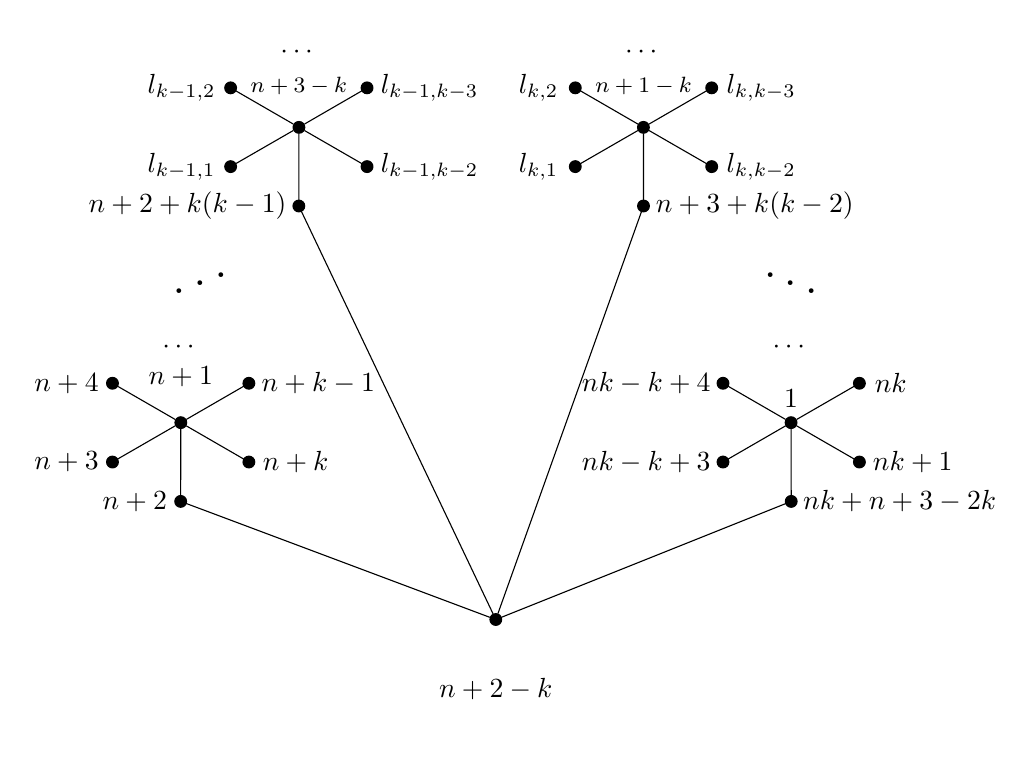
\begin{tikzpicture}[scale=1.25, every node/.style={circle, draw, fill=black, inner sep=1.5pt}]

        \node[label=below:{$n + 2 - k$}] (central) at (0, -2) {};

        \def\k{6} % Number of leaves in each star graph
        \def\leafradius{0.8} % Radius of the circular arrangement of leaves

        \node[label=above:{$n + 1$}] (b1) at (-3.2, 0) {};
        \node[label={[label distance = -0.25cm]above:{\footnotesize $n + 3 - k$}}] (b2) at (-2, 3) {};
        \node[label={[label distance = -0.25cm]above:{\footnotesize $n + 1 - k$}}] (b4) at (1.5, 3) {};
        \node[label=above:{$1$}] (b3) at (3, 0) {};

        \foreach \j in {1,...,\k} {
          \pgfmathsetmacro\leafangle{-90 - 360/\k * (\j-1)}

          \coordinate (l1\j) at ($(b1) + (\leafangle:\leafradius)$);
          \coordinate (l2\j) at ($(b2) + (\leafangle:\leafradius)$);
          \coordinate (l3\j) at ($(b3) + (\leafangle:\leafradius)$);
          \coordinate (l4\j) at ($(b4) + (\leafangle:\leafradius)$);
        }

        \node[label=left:{$n + 2$}] at (l11) {};
        \node[label=left:{$n + 3$}] at (l12) {};
        \node[label=left:{$n + 4$}] at (l13) {};
        \node[label=right:{$n + k - 1$}] at (l15) {};
        \node[label=right:{$n + k$}] at (l16) {};

        \draw (b1) -- (l11);
        \draw (b1) -- (l12);
        \draw (b1) -- (l13);
        \draw (b1) -- (l15);
        \draw (b1) -- (l16);

        \node[label=left:{$n + 2 + k(k-1)$}] at (l21) {};
        \node[label=left:{$l_{k-1,1}$}] at (l22) {};
        \node[label=left:{$l_{k-1,2}$}] at (l23) {};
        \node[label=right:{$l_{k-1,k-3}$}] at (l25) {};
        \node[label=right:{$l_{k-1,k-2}$}] at (l26) {};

        \draw (b2) -- (l21);
        \draw (b2) -- (l22);
        \draw (b2) -- (l23);
        \draw (b2) -- (l25);
        \draw (b2) -- (l26);

        \node[label=right:{$nk + n + 3 - 2k$}] at (l31) {};
        \node[label=left:{$nk - k + 3$}] at (l32) {};
        \node[label=left:{$nk - k + 4$}] at (l33) {};
        \node[label=right:{$nk$}] at (l35) {};
        \node[label=right:{$nk + 1$}] at (l36) {};

        \draw (b3) -- (l31);
        \draw (b3) -- (l32);
        \draw (b3) -- (l33);
        \draw (b3) -- (l35);
        \draw (b3) -- (l36);

        \node[label=right:{$n + 3 + k(k-2)$}] at (l41) {};
        \node[label=left:{$l_{k,1}$}] at (l42) {};
        \node[label=left:{$l_{k,2}$}] at (l43) {};
        \node[label=right:{$l_{k,k-3}$}] at (l45) {};
        \node[label=right:{$l_{k,k-2}$}] at (l46) {};

        \draw (b4) -- (l41);
        \draw (b4) -- (l42);
        \draw (b4) -- (l43);
        \draw (b4) -- (l45);
        \draw (b4) -- (l46);

        \foreach \j in {1,...,4} {
          \pgfmathsetmacro\dotangle{90}
          \node[draw=none, fill=none] at ($(b\j) + (\dotangle:0.95*\leafradius)$) {\textbf{$\cdots$}};
        }

        \draw (central) -- (l11);
        \draw (central) -- (l21);
        \draw (central) -- (l31);
        \draw (central) -- (l41);

        % Optional: add dots to indicate missing parts in the middle
        \node[draw=none,fill=none] at (-3,1.5) {\huge{\reflectbox{$\ddots$}}};
        \node[draw=none,fill=none] at (3,1.5) {\huge{$\ddots$}};

      \end{tikzpicture}
    \end{adjustbox}
    \caption{The labeling $f$ of the $B(n, k)$ tree}
    \label{fig:B(n,k)2}
  \end{figure}
  First, we show that each vertex of the $B(n, k)$ tree is labeled by a distinct element of $[nk + 1]$.
  Obviously, vertices $c_n, \ldots, c_k, r, c_1, \ldots, c_{k-1}$ are labeled by the distinct elements of $[n + 1]$. Now we discuss the labels of all other vertices $v \in \mathcal{B}$.
  For $1 \le i < k$, the vertex $a_i$ is labeled by $f(a_i) = n + 2 -k + ki$. We can see that then
  $$
  n + 3 -k + (k - 1) i - f(a_i) = 1-i \le 0
  $$
  and
  $$
  n+1 + (k-1)i  - f(a_i) = k-1-i \ge 0.
  $$
  For $k \leq i \leq n$, that is $k \leq i \leq 2k - 2$ since we have $k \leq \frac{n}{2} + 1$,  the vertex $a_i$ is labeled by $f(a_i) = n + 3 - 2k + ki$. We can see that then
  $$
  n + 3 -k + (k - 1) i - f(a_i) = k - i \le 0
  $$
  and
  $$
  n+1 + (k-1)i  - f(a_i) = 2k -2 i \ge 0.
  $$
  Therefore, for $i \in [n]$, the vertices of $\mathcal{B}_i$ are labeled by the distinct elements of
  $$
  \mathcal{F}(\mathcal{B}_i) = \{n + 3 -k + (k - 1) i, \dots, n + 1 + (k - 1) i\}.
  $$
  We also have that $\mathcal{F}(\mathcal{B}_i) \cap \mathcal{F}(\mathcal{B}_{i + 1}) = \emptyset$ since
  \begin{equation}\label{lab_bi2}
    \mathcal{F}(\mathcal{B}_{i + 1}) = \{n + 2 + (k - 1) i, \ldots, n + k + (k - 1) i\}
  \end{equation}
  and thus we have
  $$
  \min{\mathcal{F}(\mathcal{B}_{i + 1})} - \max{\mathcal{F}(\mathcal{B}_{i})} = n + 2 + (k - 1) i - ( n + 1 + (k - 1) i) = 1.
  $$
  Therefore,
  \begin{equation}\label{lab_b2}
    \begin{array}{lcl}
      \mathcal{F}(\mathcal{B}) & = & \mathcal{F}(\mathcal{B}_1) \cup \cdots \cup \mathcal{F}(\mathcal{B}_{n}) = \\ & = &
      \{n+2, \ldots n+k\} \cup \cdots \cup \{nk-k+3, \ldots , nk+1\} = \\
      & = & \{ n + 2, n + 3, \dots, nk + 1\},\\
    \end{array}
  \end{equation}
  and we conclude that the vertices of the $B(n,k)$ tree are labeled with distinct elements of $[nk + 1]$.

  Now we show that the labeling $f$ is graceful. The vertices of $\mathcal{B}_i$ are labeled by distinct elements of (\ref{lab_b2}). We will look at 2 cases.
  \begin{enumerate}
    \item If $i < k$, then  $f(c_i) = n + 2 - i$ and we have that
      $$
      \mathcal{F}^*(E(S_k^i)) = \{ f^*(c_i v) = |f(c_i) - f(v)| \, : \, v \in \mathcal{B}_i \}
      = \{ki + 1 - k , \ldots, k i - 1\}.
      $$
      In addition, $f^*(r a_i) = k i$, so the edges of one branch of the $B(n,k)$ tree are labeled by the distinct elements of
      $$
      \{ki + 1 - k , \ldots, k i\}.
      $$
      So, we have that the edges of all branches for $i < k$ are labeled by the distinct elements of
      $$
      \{1, 2, \dots, k(k - 1)\}.
      $$
    \item If $i \geq k$, then $f(c_i) = n + 1 - i$, and we have
      $$
      \mathcal{F}^*(E(S_i)) = \{ki + 2 - k , \ldots, k i\}.
      $$
      Also, then  $f^*(r a_i) = k (i - 1) + 1$. so the edges of one branch of the $B(n,k)$ tree are labeled by the distinct elements of
      $$
      \{ki + 1 - k , \ldots, k i\}.
      $$
      So, we have that the edges of all branches for $i \geq k$ are labeled by the distinct elements of
      $$
      \{k (k - 1) + 1, \ldots, nk\}.
      $$
  \end{enumerate}
  Therefore, the edges of the $B(n,k)$ tree are labeled by the distinct elements of $[nk]$, and $f$ is a graceful labeling.

  Finally, we need show to that $f$ is an $\alpha$-labeling.  We can see that $\alpha = n + 1$ since $f^*(ra_n) = |n + 1 - (n + 2)| = 1$. Following (\ref{lab_b2}) we have that $f(v) \ge \alpha$, therefore for every edge $c_i v$, $i \in [n]$, $v \in \mathcal{B}_i$, it holds that $f(c_i) \le n + 1 = \alpha < f(v)$. Finally, for the edges $r a_i$, $i \in [n]$, we have $f(r) = n + 2-k \leq \alpha < f(a_i)$. Therefore, we conclude that $f$ is an $\alpha$-labeling of the $B(n, k)$ tree.
\end{proof}

The results of the previous two theorems can be combined as follows.
\begin{corollary}
  The $B(n, k)$ tree is $\alpha$-labelable for all $n \geq 3$ and $k \geq \frac{n}{2} + 1$.
\end{corollary}

\section{Non-existence results}

\begin{theorem}
  The $B(n, k)$ tree is not $\alpha$-labelable for all $n \geq 3$ and $1 < k \le \frac{n}{2}$.
\end{theorem}

\begin{proof}
  All $B(n, k)$ trees are graceful~\cite{SJ09, SJ09b}. Assume there exists a graceful labeling $f$ such that $f \in \mathcal{P}(n, k)$, i.e. $f$ is a principal $\alpha$-labeling of the $B(n, k)$ tree. There are 2 possible types of $\alpha$-labelings in $\mathcal{P}(n, k)$

  Since $f \in \mathcal{P}(n, k)$, we have that $f(r) \le \lfloor{\frac{n}{2}}\rfloor + 1$ and, without loss of generality, we have
  $$
  f(c_i) =
  \begin{cases}
    i, & i < f(r) \\
    i + 1, & i \ge f(r)
  \end{cases}
  $$
  We know that $\mathcal{F}(RC) = [n + 1]$ since $f \in \mathcal{P}(n, k)$ and therefore $f(a_i) \ge n + 2$ for all $i \in [n]$. Thus, we also have that $$f^*(ra_i) = f(a_i) - f(r) \ge n + 2 - \left\lfloor \frac{n}{2} \right\rfloor - 1 \ge n + 1 - \frac{n}{2} = \frac{n}{2} + 1 > k.$$

  Thus, all the edges $vw$ for which $f^*(vw) \le k$, must be from $S_k^1 \cup S_k^2 \cup \dots \cup S_k^n$, i.e. must be of the form $c_i v$ where $v \in \mathcal{B}_i$. We will use the notation $v^{(x)} c_{i(x)}$ for the edge for which $f^*(v^{(x)} c_{i(x)}) = x$.

  Let us examine $v^{(1)} c_{i(1)}$. Since, we know all vertices that have labels in $[n + 1]$, we know that $f(v^{(1)}) \ge n + 2$. Therefore, we have
  \begin{equation*}
    1 = f^*(v^{(1)} c_{i(1)}) = f(v^{(1)}) - f(c_{i(1)}) \ge n + 2 - f(c_{i(1)}) \Rightarrow f(c_{i(1)}) \ge n + 1.
  \end{equation*}
  Therefore, $v^{(1)} \in \mathcal{B}_n$, since $f(c_n) = n + 1$ and $f(c_i) \le n$ for all $i \in [n-1]$. Now, we will show that $\mathcal{B}_n = \{v^{(1)}, v^{(2)}, \dots, v^{(k-1)}\}$, by induction.

  Let us suppose that we have that $V_{m-1} = \{v^{(1)}, v^{(2)}, \dots, v^{(m-1)}\} \subseteq \mathcal{B}_n$ for some $m \in [k - 2]$. Then, we know that $\mathcal{F}(V_{m-1}) = \{n + 2, n + 3, \dots, n + 1 + m - 1\}$, and the smallest vertex label we haven't yet found is $n + 1 + m - 1 + 1 = n + m + 1$, and therefore $f(v^{(m)}) \ge n + m + 1$. Furthermore, we have

  \begin{equation*}
    m = f^*(v^{(m)} c_{i(m)}) = f(v^{(m)}) - f(c_{i(m)}) \ge n + m + 1 - f(c_{i(1)}) \Rightarrow f(c_{i(1)}) \ge n + 1.
  \end{equation*}

  Thus, $v^{(m)} \in \mathcal{B}_n$ since $f(c_n) = n + 1$ and $f(c_i) \le n$ for all $i \in [n-1]$. Furthermore, now we know that $\mathcal{B}_n = \{v^{(1)}, v^{(2)}, \dots, v^{(k-1)}\}$, and $f(v^{(i)}) = n + 1 + i$ for all $i \in [k - 1]$.

  Let us now examine $v^{(k)} c_{i(k)}$. Since $\mathcal{F}(RC) = [n + 1]$, and $\mathcal{F}(\mathcal{B}_n) = \{n+2,n+3, \dots, n + k\}$, we know that $f(v^{(k)}) \ge n + k + 1$, and we also know that $f(c_{i(k)}) \le n$. Therefore, we have:
  $$
  f^*(v^{(k)} c_{i(k)}) = f(v^{(k)}) - f(c_{i(k)}) \ge n + k + 1 - n = k + 1
  $$
  Therefore, we don't have an edge $vw$ for which $f^*(vw) = k$ and we conclude that $f$ is not even a graceful labeling. Thus, we know that $P(n, k) = 0$ for every $n \ge 2$ and therefore the $B(n, k)$ tree is not $\alpha$-labelable for all $n \geq 3$ and $1 < k \le \frac{n}{2}$ by Corollary \ref{cor:alpha-labeling-nonexistence}.
\end{proof}

\section{Conclusion}

All of our results on the $\alpha$-labelability of the $B(n,k)$ trees are summarized in the next graph which shows whether an $\alpha$-labeling exists for $B(n, k)$.

\begin{figure}[H]
  \centering
  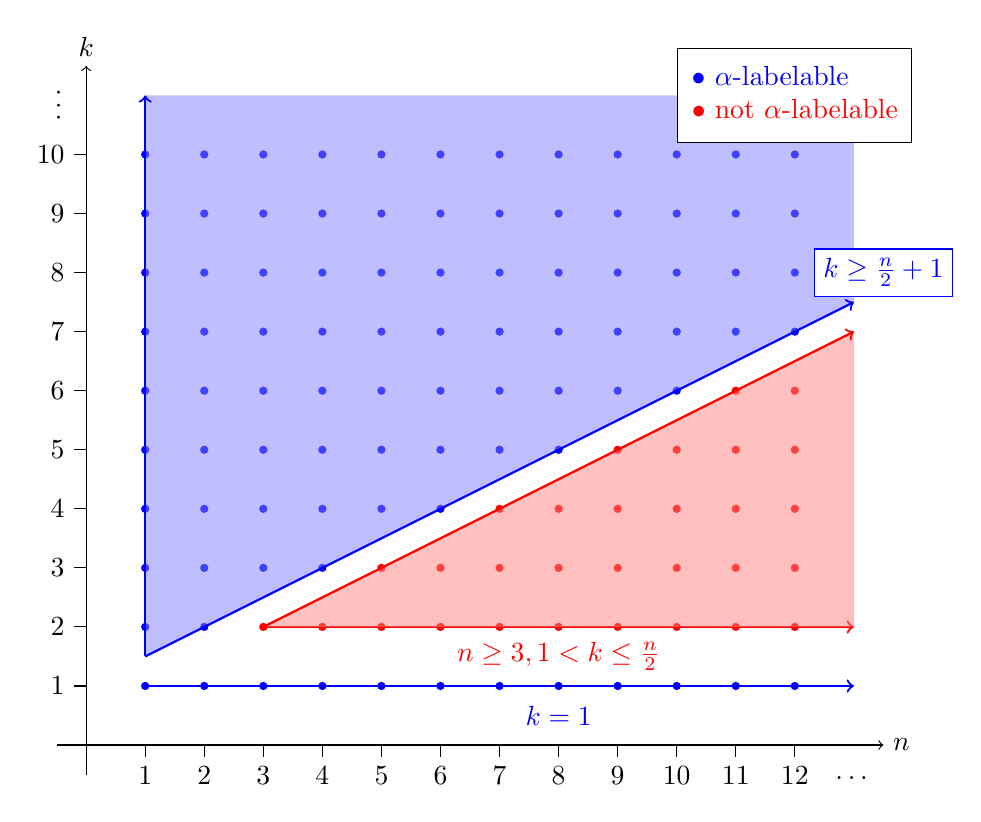
\begin{tikzpicture}[scale=0.75]
    % Draw grid points for integer lattice
    \foreach \y in {2,...,10} {
      \pgfmathparse{min(12, 2*\y-2)}
      \let\xmax\pgfmathresult
      \foreach \x in {1,...,\xmax} {
        \fill[blue] (\x,\y) circle (2pt);
      }
    }

    % Highlight the region k >= n/2 + 1
    \fill[blue!50, opacity=0.5] (1,1.5) -- (13,7.5) -- (13,11) -- (1,11) -- cycle;
    \draw[blue, thick, ->] (1,1.5) -- (13,7.5);
    \draw[blue, thick, ->] (1,1.5) -- (1,11);

    \foreach \x in {1,...,12} {
      \fill[blue] (\x,1) circle (2pt);
    }

    % Highlight the line k = 1
    \draw[blue, thick, ->] (1,1) -- (13,1);

    \foreach \x in {3,...,12} {
      \fill[red] (\x,2) circle (2pt);
    }

    % Highlight the line k = 1, n >= 3
    \draw[red, thick, ->] (3,2) -- (13,2);

    \foreach \x in {5,...,12} {
      \pgfmathsetmacro{\ymax}{(\x+1)/2}
      \foreach \y in {3,...,\ymax} {
        \fill[red] (\x,\y) circle (2pt);
      }
    }

    % HIghlight the unknown region
    \fill[red!50, opacity=0.5] (3,2) -- (13,2) -- (13,7) -- cycle;
    \draw[red, thick, ->] (3,2) -- (13,7);

    % Draw axes
    \draw[->] (-0.5,0) -- (13.5,0) node[right] {$n$};
    \draw[->] (0,-0.5) -- (0,11.5) node[above] {$k$};

    % Axis ticks
    \foreach \x in {1,2,...,12} {
      \draw (\x,0) -- (\x,-0.2) node[below] {\x};
    }
    \node[label={[label distance = 0cm] below:{$\dots$}}] at (13, -0.2) {};

    \foreach \y in {1,2,...,10} {
      \draw (0,\y) -- (-0.2,\y) node[left] {\y};
    }
    \node[label={[label distance = 0cm, rotate=90] left:{$\dots$}}] at (-0.3, 11.35) {};

    % Labels
    \node[blue, rectangle, draw, fill=white] at (13.5,8) {$k \geq \frac{n}{2} + 1$};
    \node[blue] at (8,0.5) {$k = 1$};
    \node[red] at (8,1.5) {$n \geq 3, 1 < k \le \frac{n}{2}$};

    % Legend
    \begin{scope}[shift={(12,11.5)}]
      \node[draw, rectangle, fill=white, inner sep=5pt] at (0,-0.5) {%
        \begin{tabular}{@{}l@{}}
          \textcolor{blue}{$\bullet$} \textcolor{blue}{$\alpha$-labelable} \\
          \textcolor{red}{$\bullet$} \textcolor{red}{not $\alpha$-labelable} \\
        \end{tabular}
      };
    \end{scope}
  \end{tikzpicture}
  \caption{Existence of an $\alpha$-labeling for the $B(n, k)$ tree}
  \label{fig:labeling-graph}
\end{figure}

\bibliographystyle{model1-num-names}

\begin{thebibliography}{7}

  \bibitem{CHY97}
  Chen, Wen-Chin, Lu, Hsueh-I, Yeh, Yeong-Nan, \textit{Operations of interlaced trees and graceful trees}. Southeast Asian Bull. Math. 21 (4), 1997, 337--348.

  \bibitem{G97}
  Joseph A. Gallian, \textit{A Dynamic Survey of Graph Labeling}, Electron. J. Comb, $\#$DS6, 1997

  \bibitem{G72}
  S. W. Golomb, \textit{How to number a graph}, In Graph Theory and Computing, R. C.
  Read, ed., Academic Press, New York (1972) 23--37.

  \bibitem{MMK14}
  Munia, Afsana and Maowa, Jannatul and Kaykobad, Mohammad, \textit{A new class of Graceful Tree}. International Journal of Scientific and Engineering Research 5, 2014, 1112-1115.

  \bibitem{R77}
  A. Rosa, \textit{Labeling snakes}, Ars Combin. 3, 1977, 67--73

  \bibitem{R67}
  A. Rosa, \textit{On certain valuations of the vertices of a graph}, In: Theory of graphs (Internat. Sympos., Rome, 1966), 349--355, Gordon \& Breach, New York, 1967.

  \bibitem{SJ09}
  Sethuraman, G and Jesintha, J, \textit{All banana trees are graceful, Advances Appl}, Disc. Math 4, 53--64, 2009.

  \bibitem{SJ09b}
  Sethuraman, G and Jesintha, J, \textit{All extended banana trees are graceful}, Proc. Internat. Conf. Math. Comput. Sci 1, 4--8, 2009.

  \bibitem{SSS23}
  Simarmata, Nikson and Sandy, Ikhlas Pratama and Sugeng, Kiki Ariyanti, \textit{Graceful labeling construction for some special tree graph using adjacency matrix}, Electron. J. Graph Theory Appl. 11 (2), 2023, 343--356.

\end{thebibliography}

\end{document}
